\documentclass[11pt, letterpaper]{article}
\usepackage{graphicx} % Required for inserting images
\usepackage[margin=1.2in]{geometry}
\usepackage{hyperref} % for linking in pdf
\usepackage[sorting=none, style=ieee, backend=biber]{biblatex} %additional arguments put references in chronological order
\usepackage{listings}
\usepackage{xcolor}

% Listing style for MATLAB
\definecolor{mygreen}{RGB}{0,128,0}
\definecolor{myblue}{RGB}{0,0,255}
\lstdefinestyle{mystyle}{
    language=Matlab,
    basicstyle=\footnotesize\ttfamily,
	commentstyle=\color{mygreen},
    backgroundcolor=\color{white},
    breaklines=true,
    showspaces=false,
    showstringspaces=false,
    showtabs=false,
    numbers=left, % Add line numbers
    numberstyle=\tiny\ttfamily, % Set the style of line numbers
    stepnumber=1, % Set the step between line numbers
    moredelim=[s][\color{myblue}]{\%\%}{\%\%}, % Set the style for sections marked with %%
    literate=*{\%\%}{{{\color{myblue}\%\%}}}2 % Mark %% as blue without affecting the rest of the code
}

\graphicspath{ {./images/} }

\addbibresource{MachineVisionBib.bib}

\title{Machine Vision Coursework}
\author{Ruairi McElhatton}
\date{May 2024}

% Everything before \begin is "preamble"
\begin{document}

\maketitle
\pagebreak

\tableofcontents

\pagebreak
\section{Task 1: Introduction to Machine Vision}

\subsection{Lab Session 1 - Part I}
In this task, we were required to create a red, green and blue (RGB) image histogram of any picture we wanted and include the original image in that too. This is depicted in figures \ref{fig:GreenSpaceImage} and \ref{fig:imageWRGBhist}. The histograms in figure \ref{fig:imageWRGBhist} show us the spread of each colour's intensity. From the blue histogram, we can see that blue is underexposed in the picture in question. We can tell this is the case due to there not being any information for the whites on the right side of the blue graph. We can describe the blue histogram here as being ``lowkey" \cite{ImageHistograms}.

The red and green histograms are a bit more spread out, but red is still a little underexposed with most of the information here being towards the left hand side. Right is more central and spread out but has more information missing than red towards the most intense part of the histogram (the right).


\begin{figure}[ht]
    \centering
    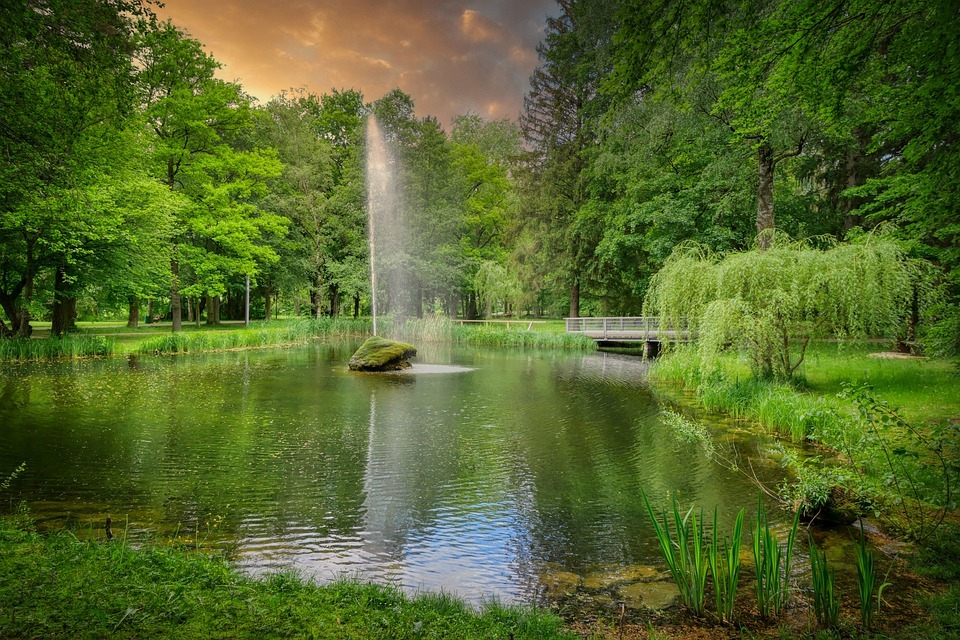
\includegraphics[width=0.5\linewidth]{Lab 1/GreenSpaceImage.png}
    \caption{Original image}
    \label{fig:GreenSpaceImage}
\end{figure}

\begin{figure}[ht] % [ht] is supposed to put the figure at this point in the document
    \centering
    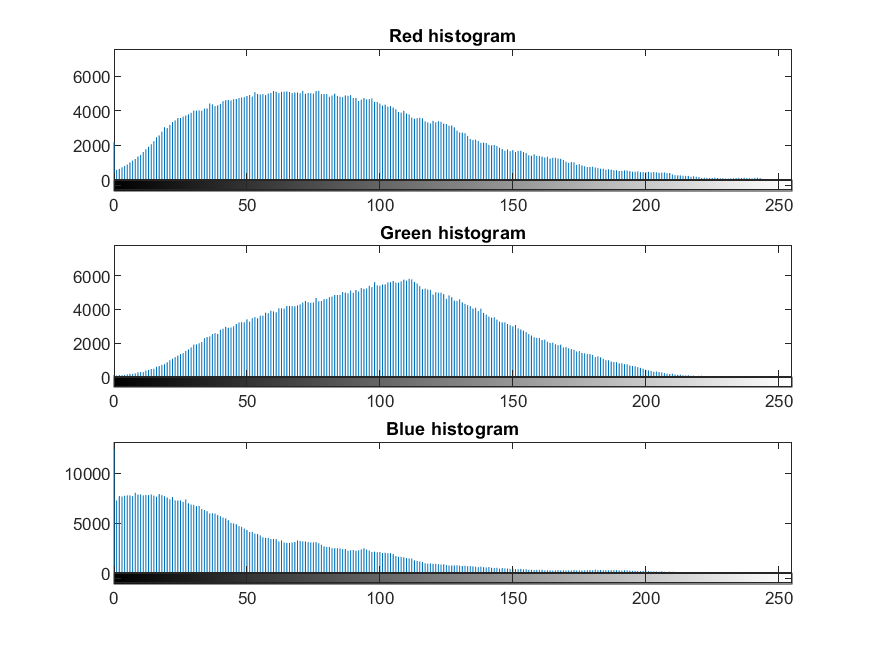
\includegraphics[width=0.6 \linewidth]{Lab 1/imageWRGBhist.png}
    \caption{RGB histograms of original image}
    \label{fig:imageWRGBhist}
\end{figure}

Overall, based off the histograms we can tell that there is less blue in the original image compared to the other two colours. 


\subsection{Lab Session 1 - Part II}
This section goes into more detail around edge detection algorithms including Sobel, Prewitt and Canny. I decided to use a new image in this section which shows a fruit stall. This can be seen in figure \ref{fig:Fruits}.

\begin{figure}[ht]
    \centering
    \includegraphics[width=0.25\linewidth]{Lab 1/imageFruits.png}
    \caption{Fruit stall image}
    \label{fig:Fruits}
\end{figure}

\subsubsection*{Enhancement contrast}
The first part of this section was to analyse the original image histogram, seen in the first row of figure \ref{fig:ImagesHistogramsEnhancedHistEq} and decide which method of enhancement would be best to increase contrast. Due to \ref{fig:ImagesHistogramsEnhancedHistEq} hinting that the image may be a little underexposed, I thought \textit{histogram equalisation} would be the best option for image enhancement due to the method being known for its ability to improve image contrast.
I thought this would be a better option than \textit{gamma correction} for example, which is more useful when trying to change the overall image intensity, without making a difference to contrast.

The second part of this section was to see if image enhancement using \textit{histogram equalisation} worked well. To use this method, the image first had to be converted to a greyscale image. The results of using the method can be seen in figure \ref{fig:ImagesHistogramsEnhancedHistEq}.

\begin{figure}[ht]
  \centering
  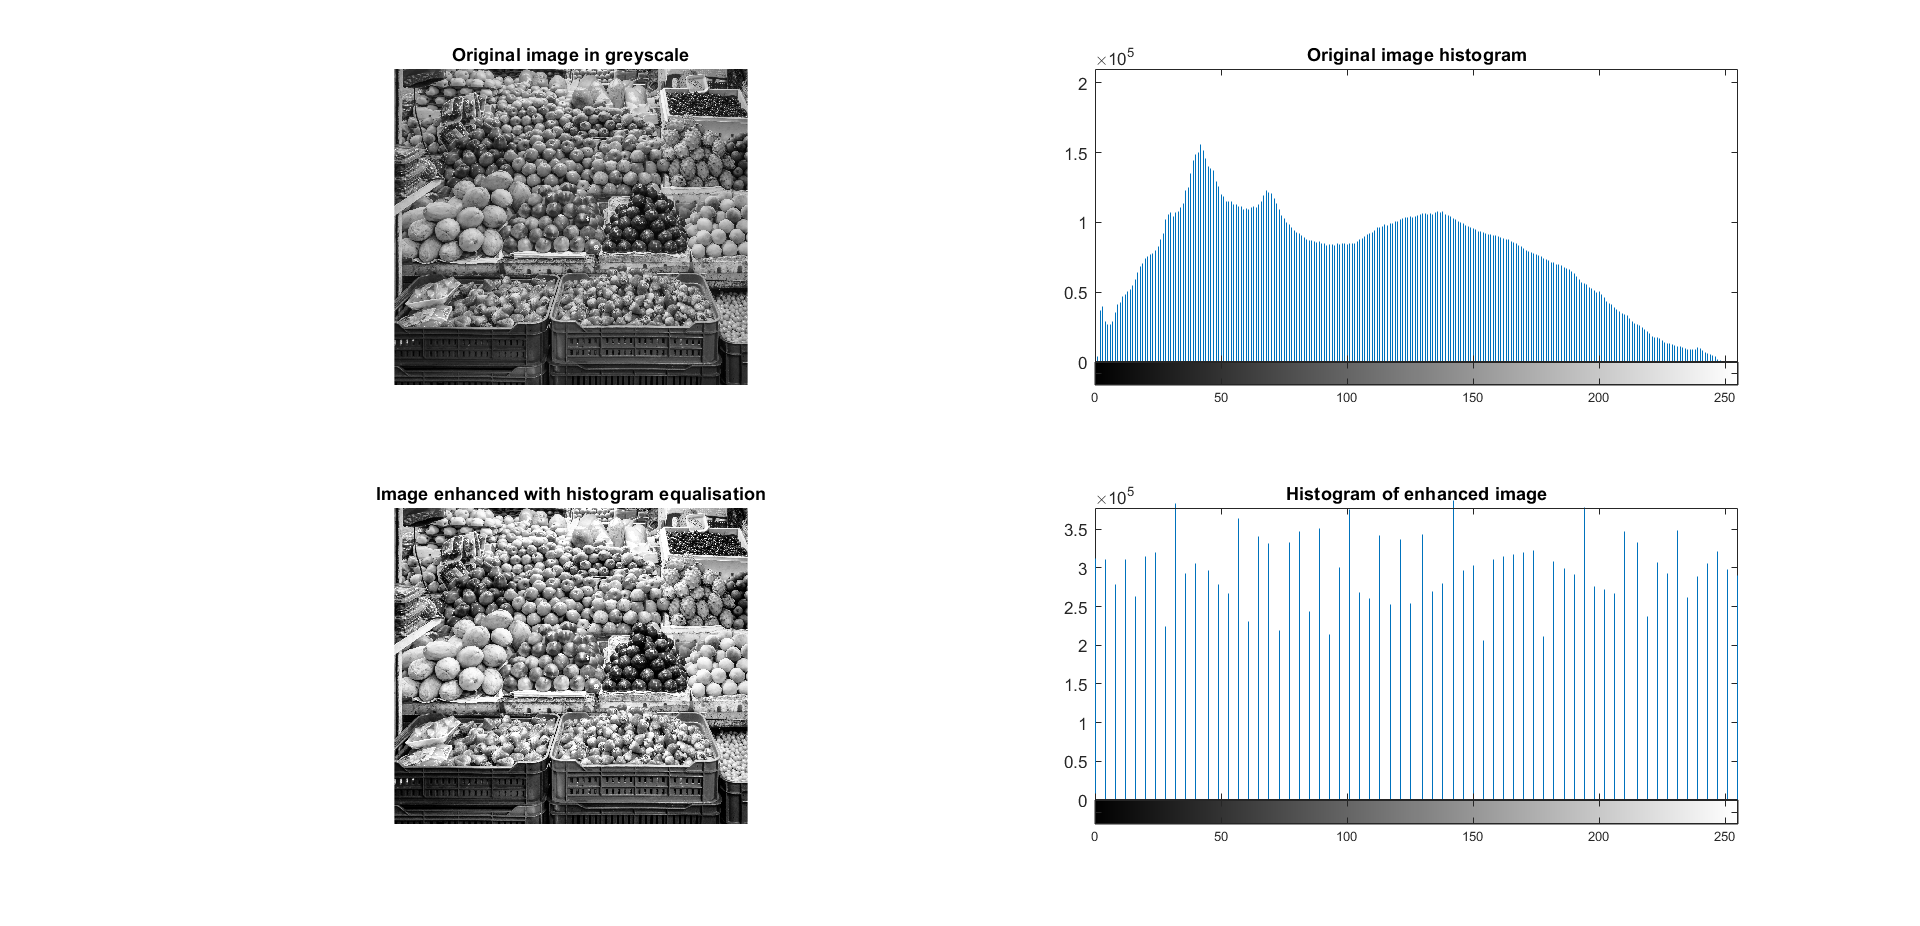
\includegraphics[width=1\linewidth]{Lab 1/ImagesHistogramsEnhancedHistEq.png}
  \caption{Image and histogram compared to histogram equalisation}
  \label{fig:ImagesHistogramsEnhancedHistEq}
\end{figure}

As we can see in \ref{fig:ImagesHistogramsEnhancedHistEq}, the intensity of the image histogram is more spread out after \textit{histogram equalisation} which means it has enhanced image quality and it will be better fit to the purposes of edge detection and segmentation. Whether it is a better image in general is a subjective view when it comes to photographs.

The next part of comparing image enhancement techniques was to look at \textit{gamma correction}. The results of this are shown in the same format as the \textit{histogram equalisation} method and are seen in figure \ref{fig:ImagesHistogramsEnhancedGammaCorrection}. I settled on gamma = 0.7 as any lower and the image intensity would be too high, creating an image which looked ``overexposed''.

\begin{figure}[ht]
  \centering
  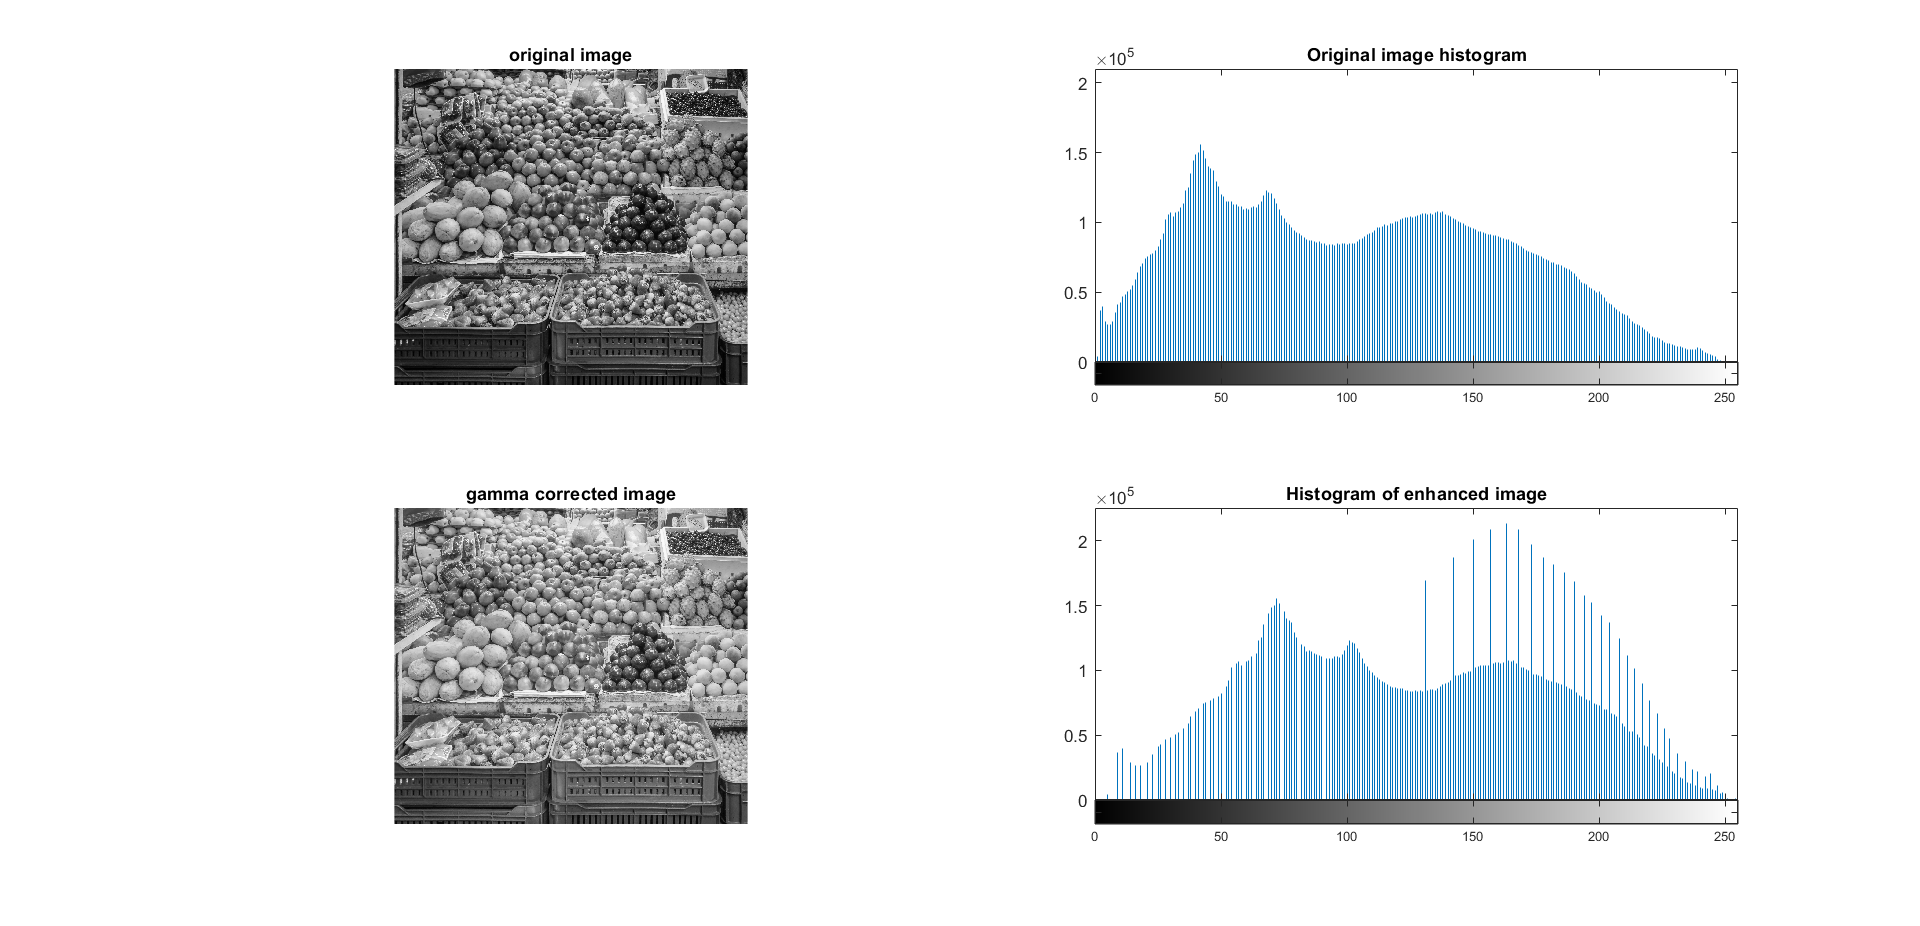
\includegraphics[width=1\linewidth]{Lab 1/ImagesHistogramsEnhancedGammaCorrection.png}
  \caption{Image and histogram compared to gamma correction}
  \label{fig:ImagesHistogramsEnhancedGammaCorrection}
\end{figure}

After seeing these two types of image enhancement in action, my initial belief that \textit{histogram equalisation} would be better for image enhancement was confrimed as correct.

\subsubsection*{Images with different types of noise and image denoising}
The next variable to test was how different types of noise could influence edge detection. The two types of noise we were to synthesise the images with were Salt and Pepper noise and Gaussian noise. 

\begin{figure}[ht]
    \centering
    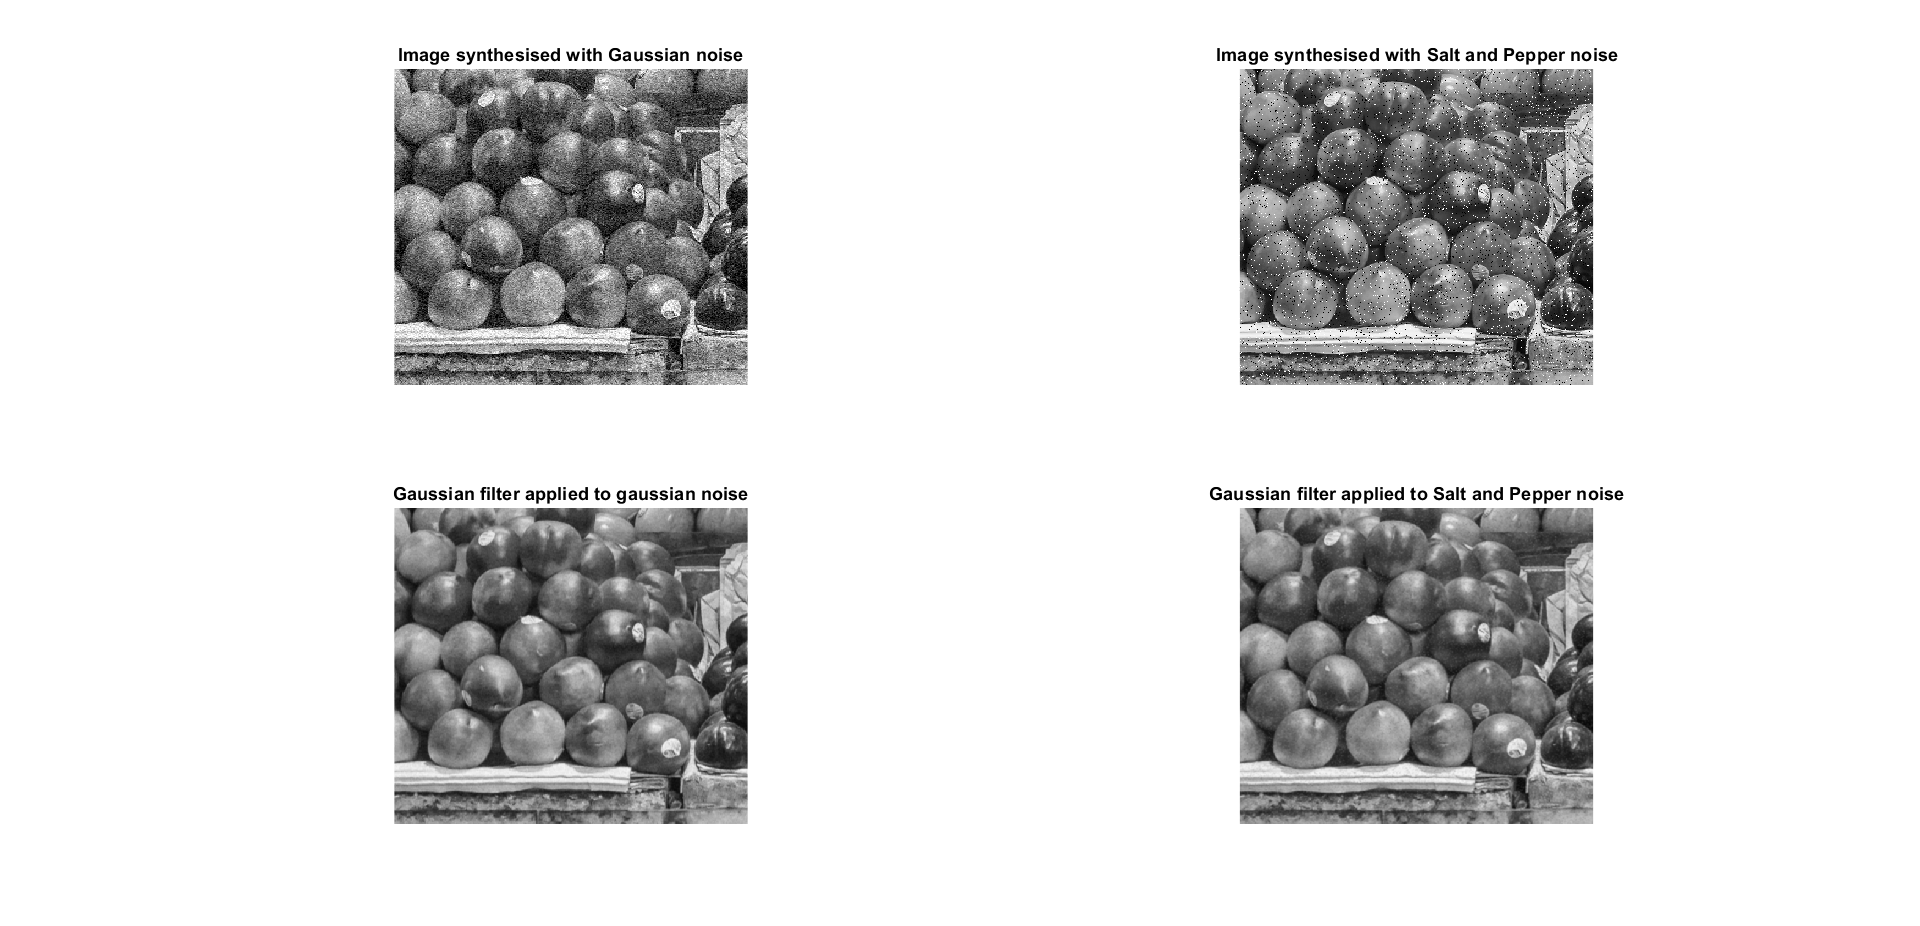
\includegraphics[width=1\linewidth]{Lab 1/NoiseSynthesisedRemovedWithGauss.png}
    \caption{Fruit image with noise}
    \label{fig:NoiseSynthesisedRemovedWithGauss}
\end{figure}

In figure \ref{fig:NoiseSynthesisedRemovedWithGauss} we can see the effect of noise on the image of the fruit (figure \ref{fig:Fruits}). The Gaussian noise makes the photograph look a bit like it has been painted, whilst it is clear why salt and pepper noise was given this name, with black (pepper) and white (salt) spots appearing on the image. The synthesised images are magnified to make the impact of the noise more visible.

We can then see what the Gaussian image filter does to both synthesised images. It makes them look almost identical to the original, but a little smoother, so the edges aren't as defined. Both of these used a Gaussian filter with standard deviation of 2. This was chosen because a \textit{s.d} that was too low meant not all the noise was removed, and a \textit{s.d} that was too high made the image very blurry.

Next, we were asked to use a median filter on the salt and pepper synthesised image. The results of before and after can be seen in figure \ref{fig:NoiseSynthesisedRemovedWithMedian}. The default filter window size of [3 3] was optimal here. At [9 9], the image was blurry, and at [1 1], the image still had the salt and pepper noise in it. 

The reason the salt and pepper noise stays there when the filter window is set so small is because when the window is small, only a very small number of neighbouring pixels are considered when filtering out noise. In this case with [1 1], the salt and pepper spots may be larger than the filter window, meaning the filter window sees the rest of the noise and only takes this into account, meaning the noise is not filtered out.

When the filter window is large, like [9 9], the image becomes blurry because all the pixels in this area filter similar colours/intensities through, meaning edges are less defined, or even lost.

\begin{figure}[ht]
  \centering
  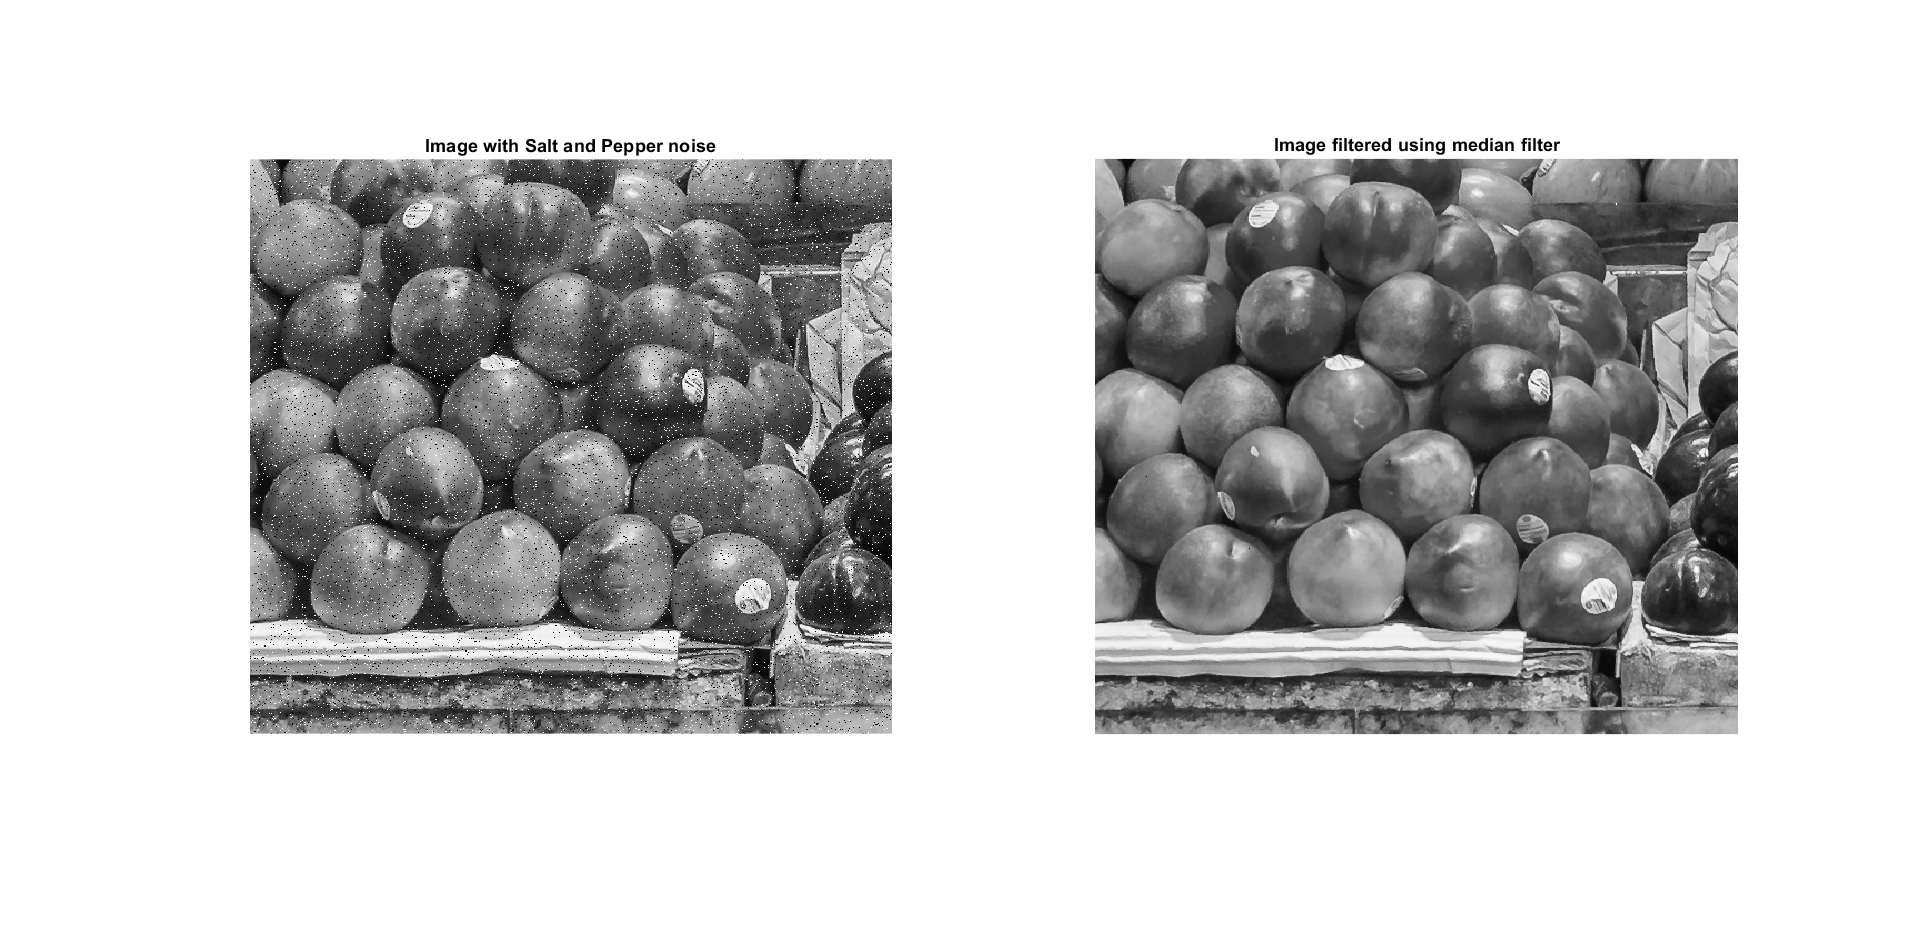
\includegraphics[width=1\linewidth]{Lab 1/NoiseSynthesisedRemovedWithMedian.png}
  \caption{Fruit image with noise}
  \label{fig:NoiseSynthesisedRemovedWithMedian}
\end{figure}

\subsubsection*{Static objects segmentation by edge detection}
The task for this part of the lab was to show results of different edge detection algorithms and see how different parameters would affect the outcome. ``An edge in an image is a significant local change in the image intensity, usually associated with a discontinuity in either the image intensity or the first derivative of the image intensity" \cite{Jain}. 

The first parameter I looked at changing was the threshold. This parameter can be adjusted to ignore edges in a picture which are not stronger than the threshold. The lower this threshold parameter is, the more white spots we will see on our image of edges. 

In figure \ref{fig:AllSegmentation} I have tried to optimise the thresholds of the Sobel and Prewitt algorithms to get a good output binary image. Both thresholds fared well when set low (0.03 out of a maximum 1) and used alongside ``nothinning", a hyperparameter available to use in MATLAB \cite{MATLABedge} which means the edge detection algorithms skip out the edge-thinning stage. The images on the first column of the figure show the binary edge image in its default state. The second column is with the optimised threshold, and the right-most column is with the optimised threshold and the ``nothinning" variable enabled.

\begin{figure}[ht]
    \centering
    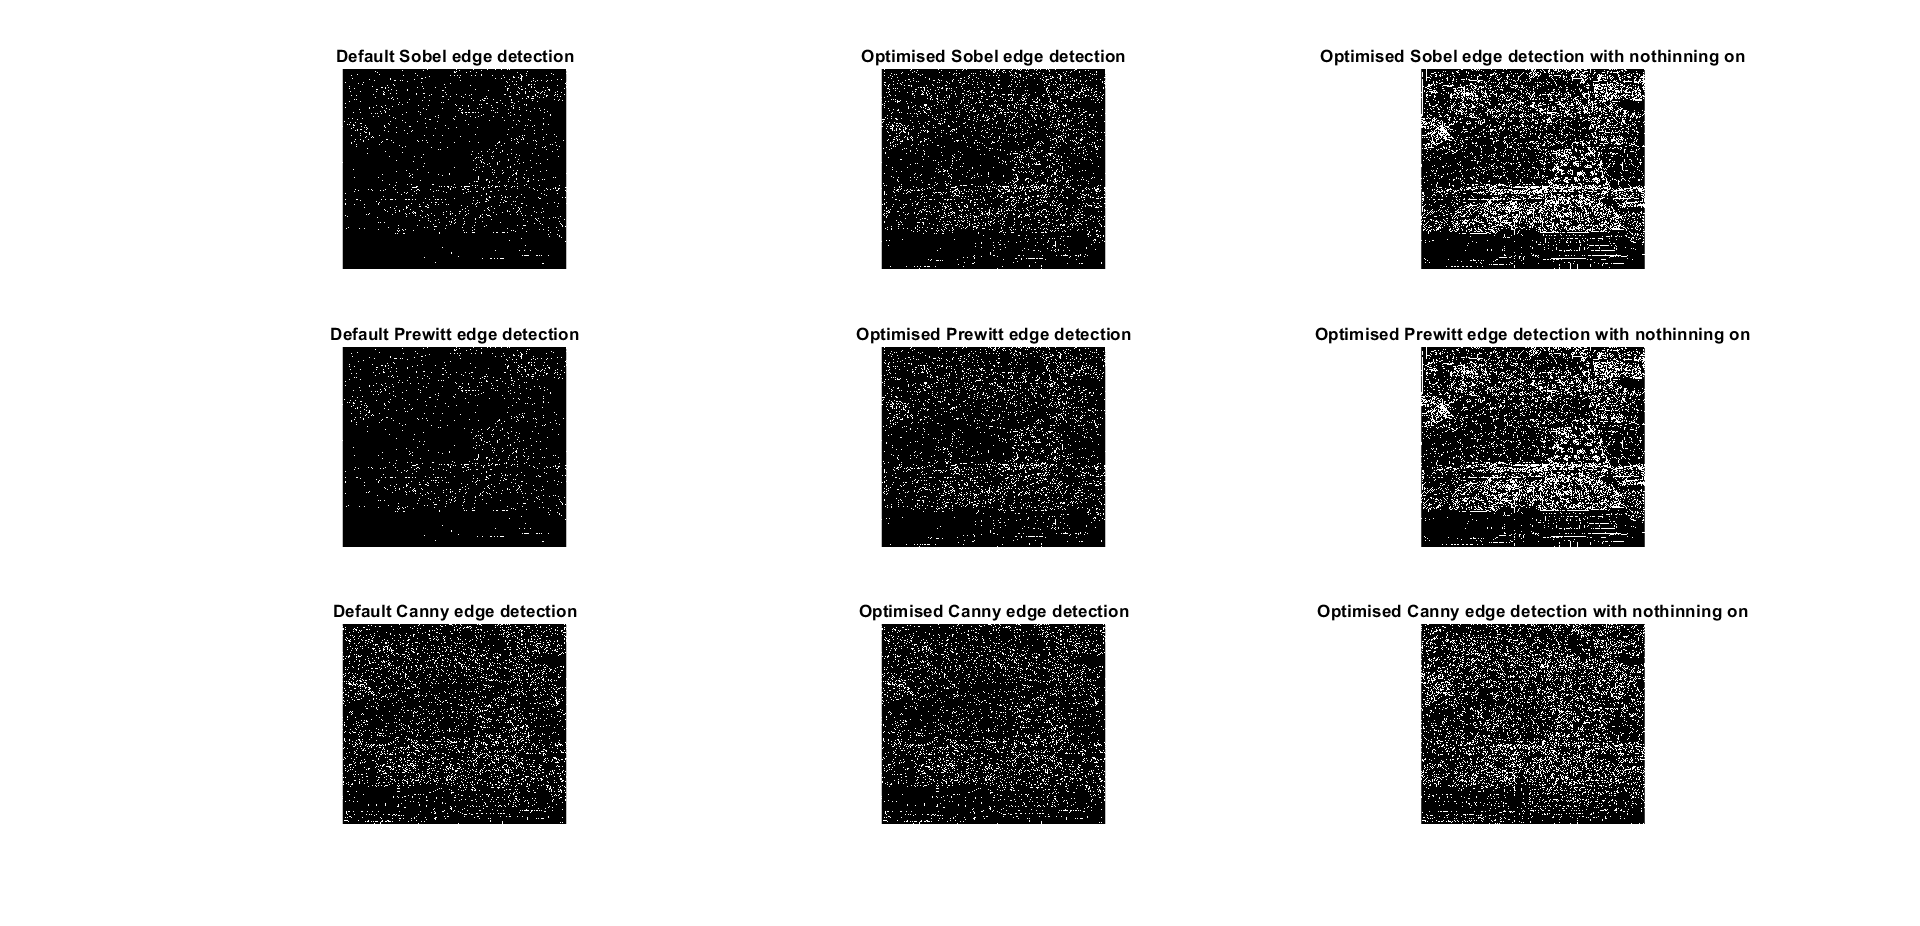
\includegraphics[width=1\linewidth]{Lab 1/AllSegmentation.png}
    \caption{Optimising segmentation algorithms}
    \label{fig:AllSegmentation}
\end{figure}

It is quite clear looking at figure \ref{fig:AllSegmentation} that the last column is the best as we can actually see the outline of shapes in the image. 

Lastly, I looked at the Canny edge detection technique along the bottom row, which required different hyperparameters to the other two. It did not yield results as good as the other two for this image, despite attempts to optimise. I chose sigma, which represents the Gaussian filter with reduced noise, to be 0.1, which is a low value. This is because setting it too high made the edges too smooth and our edge detector image almost fully black.

I then had to select two thresholds rather than one (as is the case for the other two edge detection methods). The difference being that pixels with gradient magnitudes in between the two selected thresholds are considered weak edge pixels and are included in the edge image only if they are connected to strong edge pixels (pixels which have gradient magnitudes higher than the upper threshold).

\clearpage
\section{Task 2: Optical Flow Estimation Algorithm}

\subsection{Finding Corner Points and Applying the Optical Flow Estimation Algorithm}
To begin this lab session, the ability to find corner points of an image was tested. The results of finding and highlighting a single corner from two images is seen in figure \ref{fig:markedCorners} which is programmed from the start of listing \ref{Ex2MATLABscript}. As can be seen the images, which were initially in RGB format, had to be converted into greyscale in order to find the corner points on them. I used a red square to highlight the area where the corner appears and then used the green cross to show the exact point. 

\begin{figure}[ht]
    \centering
    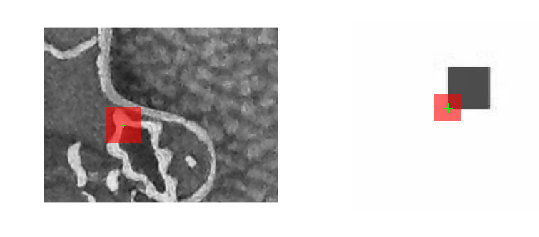
\includegraphics[width=0.75\linewidth]{Lab 2/markedCornersEdited.png}
    \caption{Square and gingerbread man marked corners}
    \label{fig:markedCorners}
\end{figure}

\subsection{Finding optical flow of the pixels between two frames}
This task involved taking two images, assumed to be consecutive frames from a video, and finding the optical flow between them, then visualising this. The result can be seen in figure \ref{fig:OpticalFlow}. As with the task visualised in figure \ref{fig:markedCorners}, the image had to be converted to gray-scale format in order to perform the task. This can be seen in lines 39-54 of \ref{Ex2MATLABscript}.

\begin{figure}[ht]
    \centering
    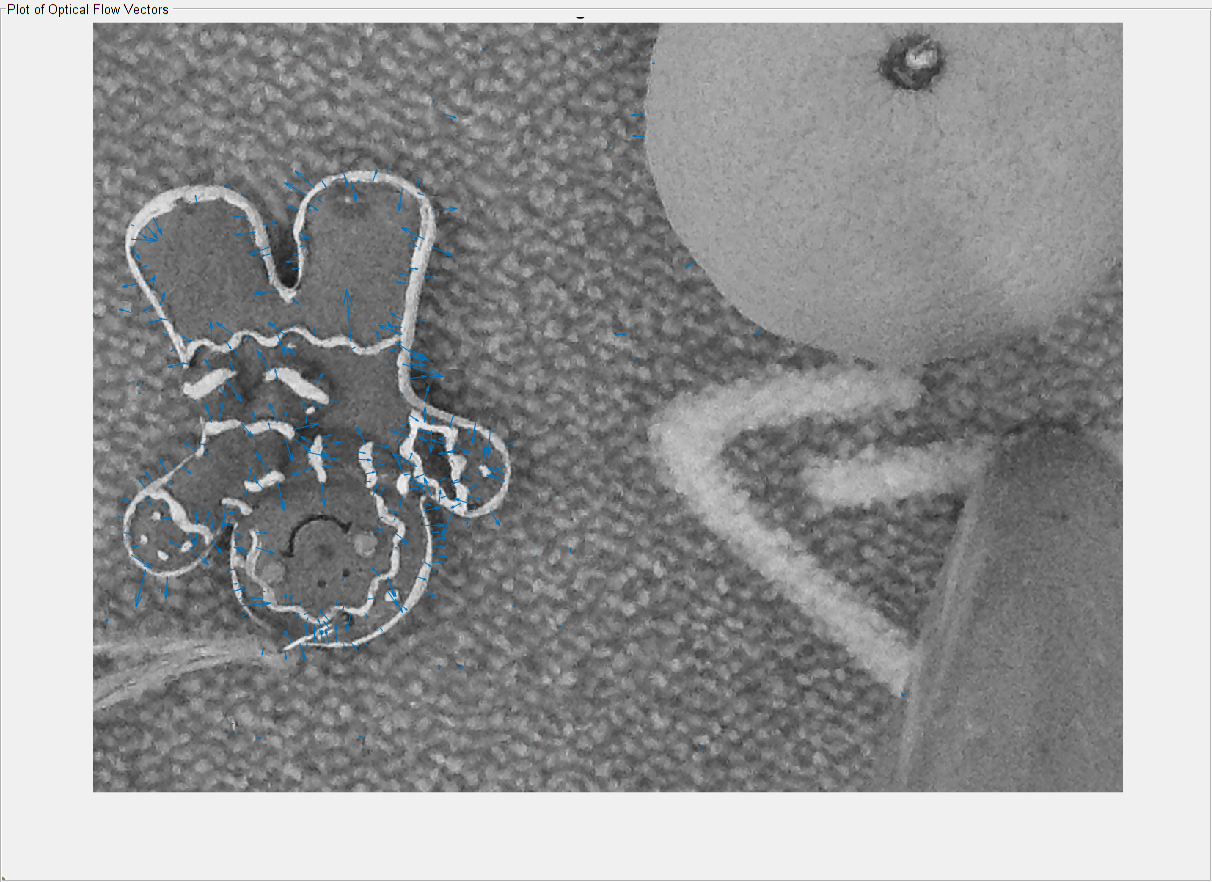
\includegraphics[width=0.75\linewidth]{Lab 2/OpticalFlowEdited.png}
    \caption{Optical flow in second gingerbread man image}
    \label{fig:OpticalFlow}
\end{figure}

The optical flow is depicted by the blue arrows on figure \ref{fig:OpticalFlow}.

\subsection{Tracking of single point using optical flow algorithm in a video} 

\subsubsection*{Visualising the track and the ground truth of red square}
The tracking throughout all 150 frames of the video compared with the ground truth can be seen in figure \ref{fig:trackCorner}. The green dots represent the ground truth of where the top left corner is in the video. The red dots represent the tracked location of the top left corner of the red square. On the face of it, the tracked trajectory looks quite accurate. The green dots and red dots are close together throughout. This can be seen in lines 56-112 of \ref{Ex2MATLABscript}.

\begin{figure}[ht]
    \centering
    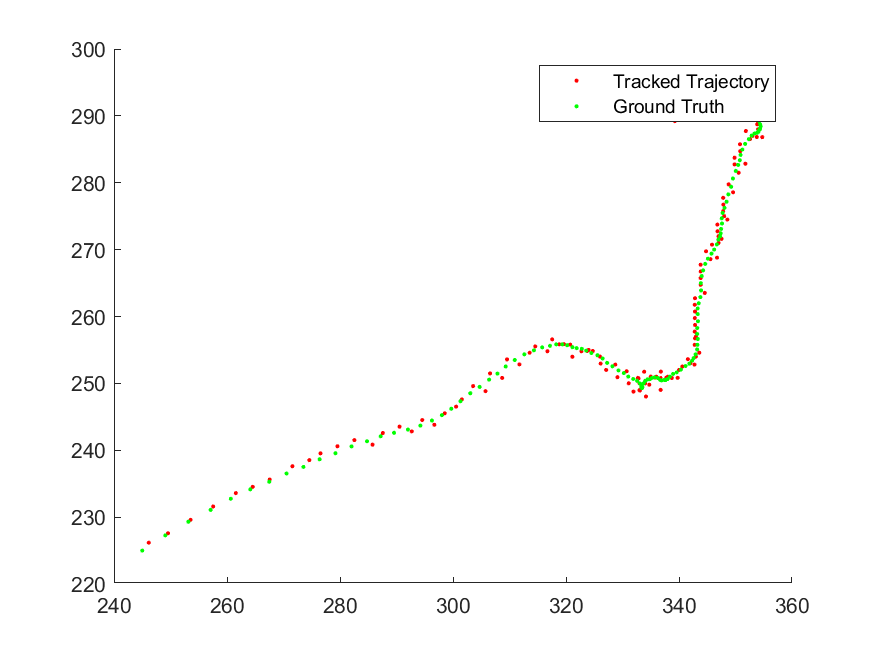
\includegraphics[width=0.75\linewidth]{Lab 2/trackCorner.png}
    \caption{Tracked path of top left corner of square vs ground truth path}
    \label{fig:trackCorner}
\end{figure}

\subsubsection*{Compute and visualise the RMSE of tracking over frames and the RMSE average value}
To see how accurate the tracked trajectory really is, the Root Mean Squared Error (RMSE) of the coordinates must be found. The basic equation for RMSE \ref{RMSE equation}
\begin{equation}\label{RMSE equation}
  RMSE = 
  \sqrt{\frac{1}{n}
      \sum_{i=1}^{N}
          \|A_{\mathrm{i}} - F_{\mathrm{i}}}|^2    
\end{equation}
is applied to both the \textit{x} and \textit{y} coordinates in our data by the MATLAB function ``rmse(F, A)''. \begin{math}A_{\mathrm{i}}\end{math} represents the tracked trajectory and \begin{math}F_{\mathrm{i}}\end{math} represents the ground truth. To find the total RMSE we then combine \begin{math}RMSE_{\mathrm{x}}\end{math} and \begin{math}RMSE_{\mathrm{y}}\end{math} in the following way:

\begin{equation}
  RMSE_{\mathrm{total}}  =
  \sqrt{RMSE_{\mathrm{x}}^2 + RMSE_{\mathrm{y}}^2}
\end{equation}

My results for this part of the lab are seen in table \ref{tab:RMSEresults}.

\begin{table}[ht]
    \centering
    \begin{tabular}{cc}
         \begin{math}RMSE_{\mathrm{x}}\end{math} & 1.0748\\
         \begin{math}RMSE_{\mathrm{y}}\end{math} & 0.6779\\
         \begin{math}RMSE_{\mathrm{total}}\end{math} & 1.2707\\
    \end{tabular}
    \caption{Corner tracking RMSEs}
    \label{tab:RMSEresults}
\end{table}

For RMSE to be useful, we need the context. In this case, the values we measure for the \textit{x} coordinates are, on average, 1.0748 pixels away from their actual point, the ground truth. When looked at in this way, it becomes clear that the tracking method used in this task is very accurate. The \textit{y} coordinates are 0.6779 pixels away from their actual point, which is even better than for \textit{x}. The combined inaccuracy is 1.2707 which is still very small. The impact of this inaccuracy will also be minimal in terms of optical flow estimation. This part of the lab is seen in MATLAB in lines 114-128 of \ref{Ex2MATLABscript}.

\clearpage
\section{Task 3: Automatic Detection of Moving Objects in a Sequence of Video Frames}

\subsection{Part I: Frame differencing approach}
The frame differencing approach works by comparing consecutive frames in a video and seeing the difference between them. If the difference in pixel intensity values for a given pixel is greater than a pre-specified threshold \begin{math}T_{\mathrm{s}}\end{math}, the pixel is considered as being a part of the foreground. One of the first steps is to make the images in question greyscale.

\begin{figure}[ht]
    \centering
    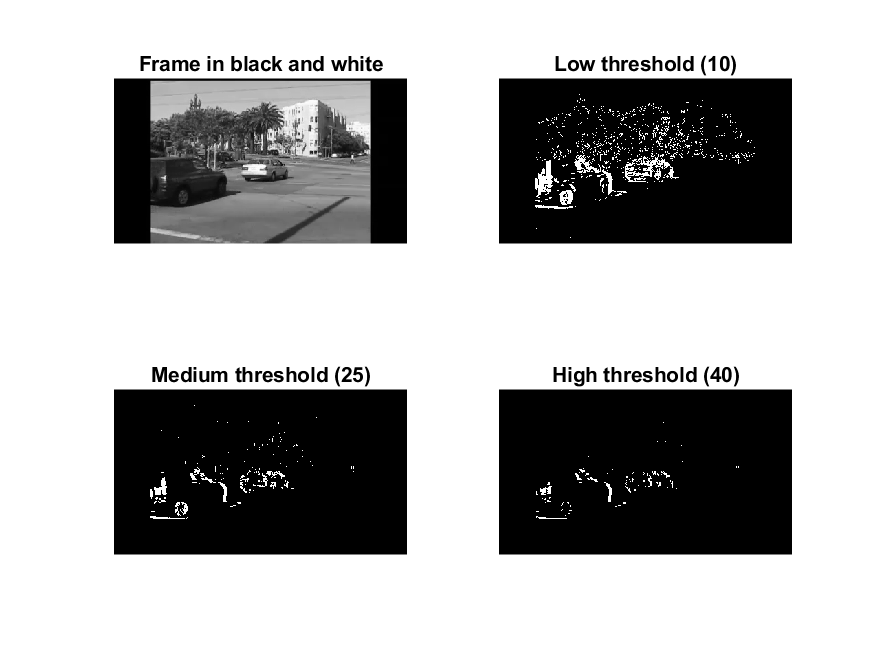
\includegraphics[width=0.75\linewidth]{Lab 3/CompareThresholds.png}
    \caption{Impact of threshold on foreground image}
    \label{fig:CompareThresholds}
\end{figure}

Figure \ref{fig:CompareThresholds} shows the aforementioned foreground in the same frame for three different thresholds. As we can see, the foreground created using a low threshold gives us more white spots than the medium and high thresholds. The reason for this is most likely because the noise within the frames of the video has an intensity greater in magnitude than 10. A partial explanation for this effect of white spots is that the trees seen on the left of the image are rustling and this leads to a change in pixel intensity from one frame to the next.

One positive with this low threshold is that when viewed in video format, we can clearly see the person crossing the road ahead of where the cars are. This cannot be seen so clearly in the higher thresholds. It may be possible to get a better result than the three seen here if we apply a filter on the foreground image created by the low threshold.

The difference seen between the medium threshold and the high threshold is less stark. There still looks to be noise in both, but the noise is more pronounced in the medium threshold foreground, as would be expected. This part of the lab is seen in lines 1-129 of \ref{Ex3MATLABscript}.

\subsection{Part II: with the Gaussian mixture approach}
In this section, the effect of Gaussian filters on images was explored. Varying different parameters on Gaussian mixtures was shown to leave us with differing results as will be shown. Setting the number of Gaussian components to one causes a black screen and it wasn't conducive to the discussion to include this, so I decided to make the ``low nGauss'' image have two Gaussian components.

Gaussian mixtures detect movement between frames by having multiple Gaussian distributions across the pixel intensity spectrum. Each pixel is allocated to a Gaussian component based on its intensity. If a pixel's intensity changes from one frame to the next by more than 2\begin{math}\sigma\end{math} from the mean (with \begin{math}\sigma\end{math} being one standard deviation) then the foreground image shows this as movement. It is similar to the frame differencing approach but the threshold here is just 2$\sigma$. 

\subsubsection*{Impact of varying number of Gaussian components}
\begin{figure}[ht]
    \centering
    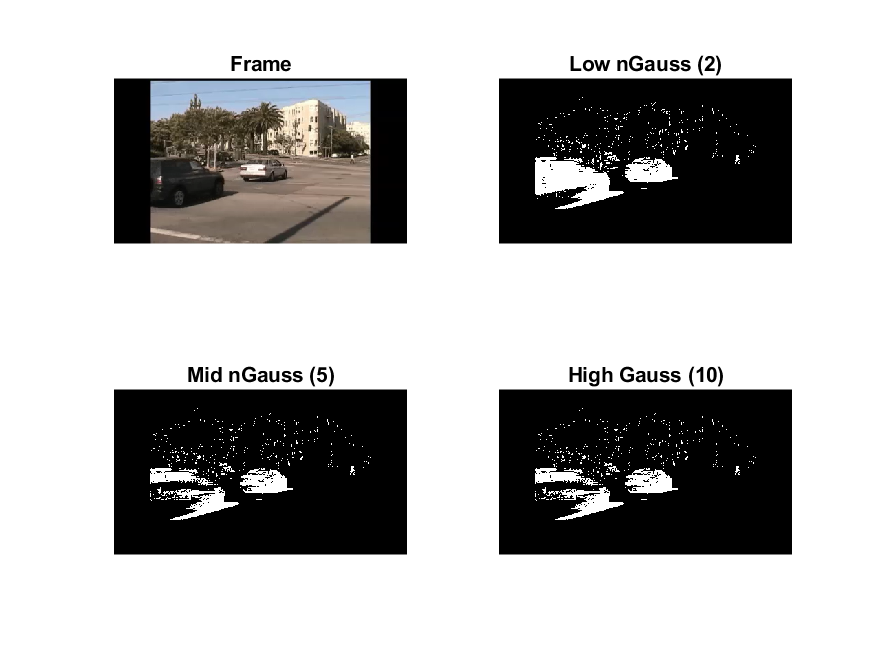
\includegraphics[width=0.75\linewidth]{Lab 3/CompareNGauss.png}
    \caption{Impact of number of Gaussian modes on the detection results}
    \label{fig:CompareNGauss}
\end{figure}

As can be seen in figure \ref{fig:CompareNGauss}, there are changes as we vary the number of Gaussian components when detecting motion from frame to frame. When changing the number of Gaussian components from two to five, the amount of noise in the foreground image is almost identical. The difference comes in the actual detection of motion. Looking at the cars in the two images, we can see that in the low nGauss image, the space that the black car takes is lighter than for the mid nGauss image. The MATLAB guidance \cite{MATLABGaussianMixtures} for the hyperparameter is minimal, but what it does say is that to model multiple background modes, the number of Gaussian components would have to be 3 or greater.

This part of the lab is seen in lines 276-419 of \ref{Ex3MATLABscript}.

\subsubsection*{Impact of varying number of frames learnt on}
\begin{figure}[ht]
    \centering
    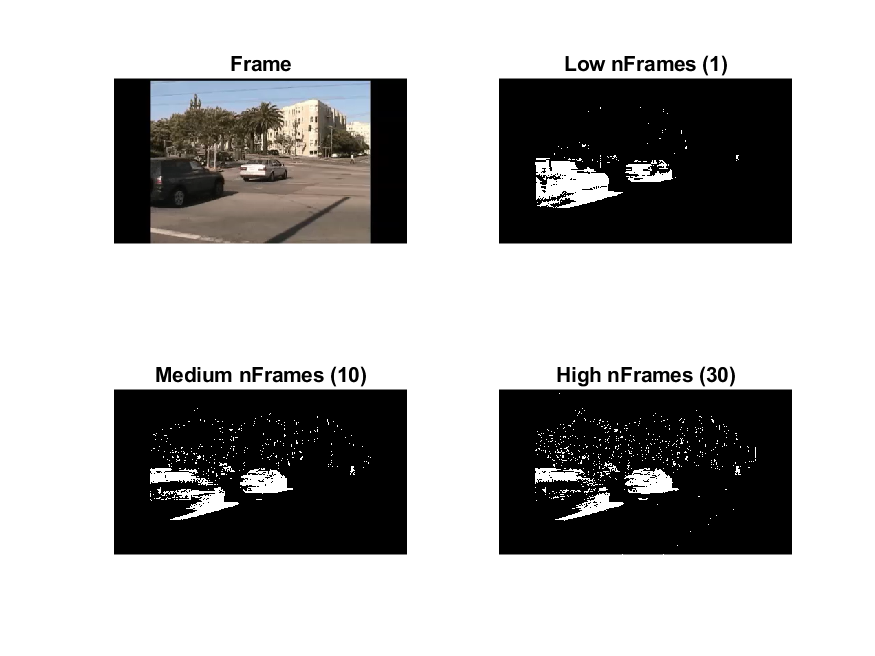
\includegraphics[width=0.75\linewidth]{Lab 3/CompareNFrames.png}
    \caption{Impact of changing number of frames learnt on detection results}
    \label{fig:CompareNFrames}
\end{figure}
It can be seen in figure \ref{fig:CompareNFrames} that as the number of frames learnt on increases, so does the noise in the image. There is a lot more white spotting towards the top of the image in the foreground image ``High nFrames'' than in ``Low nFrames''. No matter the number of frames used to train, the cars can still be seen clearly. However, a difference is seen when looking at the person crossing the road ahead of the cars. As the number of frames used to train the background model increases, so does the clarity of that figure. So there is a trafe-off. Is it preferable to have less noise but potentially miss a moving figure, or to have more noise but a clearer picture of a moving object?

In my opinion the latter, image detection with more noise but a clearer picture of the moving object, is preferable. I am confident that with some further image processing, the noise in the image could be removed whereas it would be more difficult to make a moving object in an image clearer.

This part of the code can be seen in lines 132-274 of \ref{Ex3MATLABscript}.

\pagebreak
\section{Task 4: Robot Treasure Hunting}
In this task we are given the task of ``finding the treasure" in three separate images which are seen in figure \ref{fig:threeTreasures} by using image processing techniques to follow the arrows on the images.
\begin{figure}[ht]
    \centering
    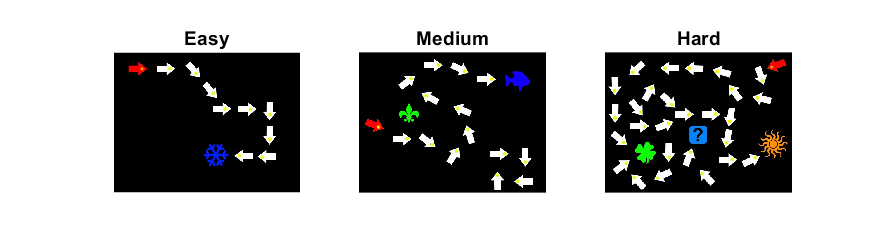
\includegraphics[width=1\linewidth]{Lab 4/threeTreasuresCropped.png}
    \caption{The three images to perform the tasks on}
    \label{fig:threeTreasures}
\end{figure}

\subsection{Binarisation and object detection}
One of the first tasks that needed to be completed was to binarise the images in preparation for using a built-in MATLAB function which identifies objects in an image. In figure \ref{fig:varyingThresholds} it can be seen what happens when we vary the threshold between 0 and 0.2. Clearly, the optimal threshold is at 0.1. This is seen implemented in line 9 of listing \ref{Ex4MATLABscript}.
\begin{figure}[ht]
    \centering
    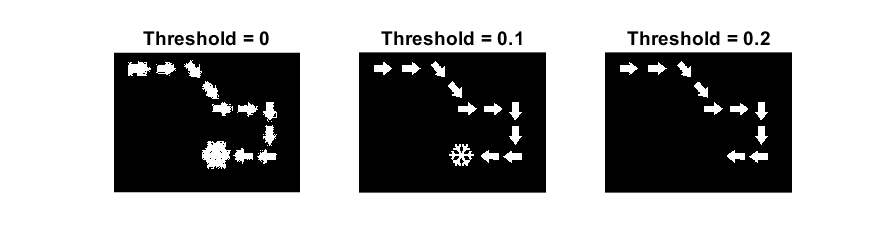
\includegraphics[width=1\linewidth]{Lab 4/varyingThresholdsCropped.png}
    \caption{Varying thresholds lead to the following}
    \label{fig:varyingThresholds}
\end{figure}
Having the threshold too high means some darker (less intense) objects within the image are not above the threshold and are therefore lost in the binary image. Having the threshold too low means that the edges of shapes are not made out very well and also noise is allowed to make it through to the binarised image. This would mean we end up with more objects than we actually have when getting onto the next couple of steps.

Once the shapes in the images have been identified, we can use the function ``bwlabel()" in line 15 of listing \ref{Ex4MATLABscript} to give each one their own number. This function outputs a matrix the same size as the image so the pixels in each shape are given a number corresponding to the shape number. This number replaces what was the intensity of that pixel on the image.

Now that each image has its own number, we can use another function ``regionprops()'', which computes different characteristics of the objects identified. This is implemented in line 19 of listing \ref{Ex4MATLABscript}

\subsection{Identifying arrows}
The next part of the task was to identify the indicies of the shapes which were arrows. I set about doing this by looking at the characteristics of the different shapes and seeing what was common between the arrows and what stood out from the other shapes. The areas of the arrows were between a range (\begin{math}1430<area<1600\end{math}) which the other shapes seen in the three images in figure \ref{fig:threeTreasures} were not. The outcome of this can be seen in figure \ref{fig:arrowFinder}. The function I made for this subtask can be seen in listing \ref{arrowFinderFunction}. The next step in the code was to find the red arrow which was our starting point by inputting the arrow indicies into the code which had been written for us.

\begin{figure}[ht]
    \centering
    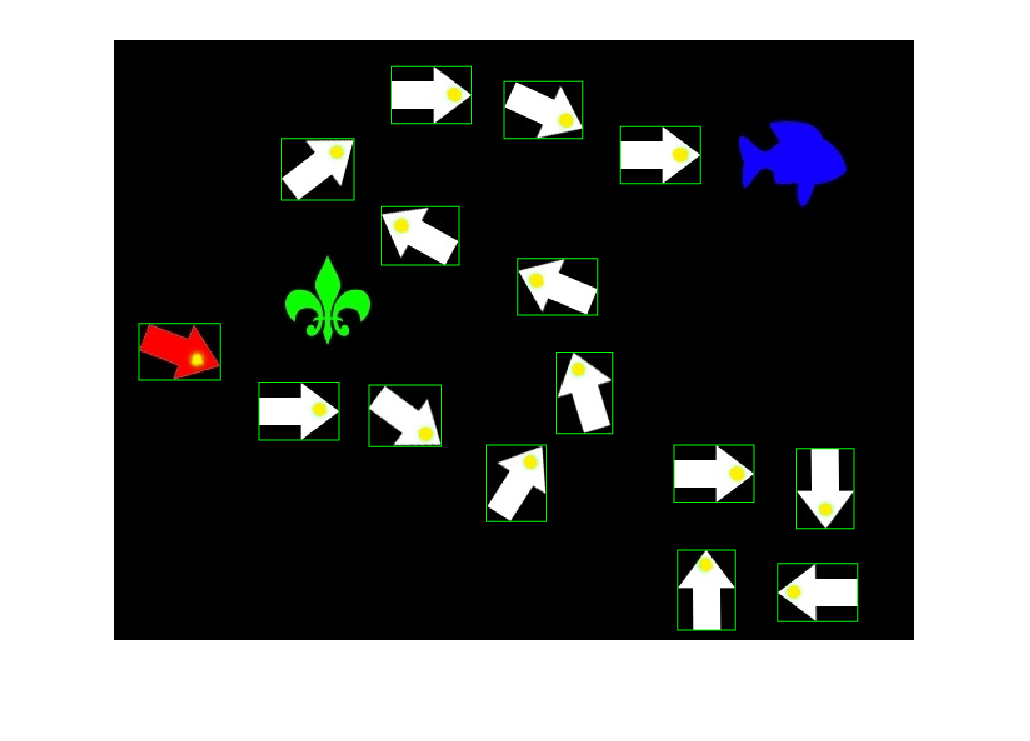
\includegraphics[width=0.75\linewidth]{Lab 4/arrowFinder.png}
    \caption{Arrows identified on image}
    \label{fig:arrowFinder}
\end{figure}

\subsection{Find the next object}
In this stage we needed to find the next object along by working out, programmatically, which way the arrows were pointing. We would follow this path until we reached the treasure. I decided to go with a solution which involved using the yellow points which can be seen on all of the arrows to create a vector pointing to the next arrow.

As can be seen in listing \ref{yellowFinderFunction}, I have created a new field within the props class for the objects. The new field represents the centroids of the yellows spots seen on the arrows. These are matched up to the corresponding arrow struct in the correct order within the function in listing \ref{yellowFinderFunction}. 

In \ref{arrowFinderFunction}, a line is drawn between the centroid of the arrow and the centroid of the yellow spot. This is then extended until it reaches the next object. If the next object is an arrow, this process is repeated. This goes on until we reach an object which is not an arrow and is therefore the treasure. 

\subsection{Visualisation of the solution}
Finally, once the path of the solution had been found and stored in an array, the visualisation code had been written for us. So all I had to do at this point was run it. The solutions for the easy, medium and hard images can be seen in figures \ref{fig:EasyVisualSolution}, \ref{fig:MediumVisualSolution} and \ref{fig:HardVisualSolution} respectively.

\begin{figure}[ht]
    \centering
    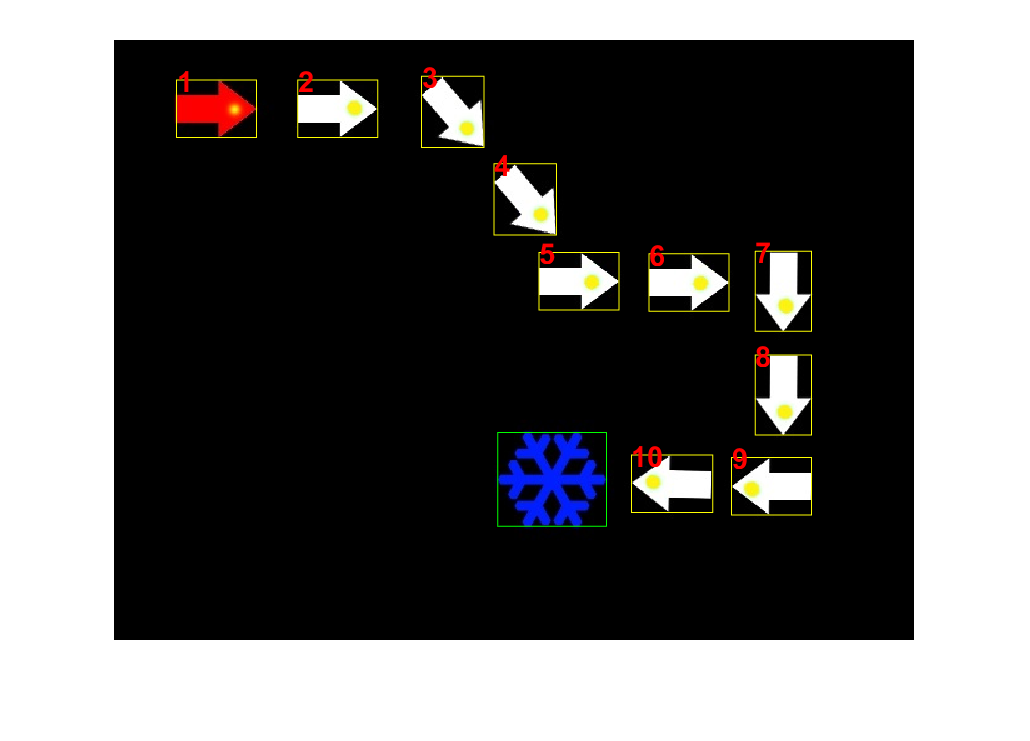
\includegraphics[width=0.75\linewidth]{Lab 4/EasyVisualSolution.png}
    \caption{Visualisation of easy treasure hunting}
    \label{fig:EasyVisualSolution}
\end{figure}

\begin{figure}[ht]
    \centering
    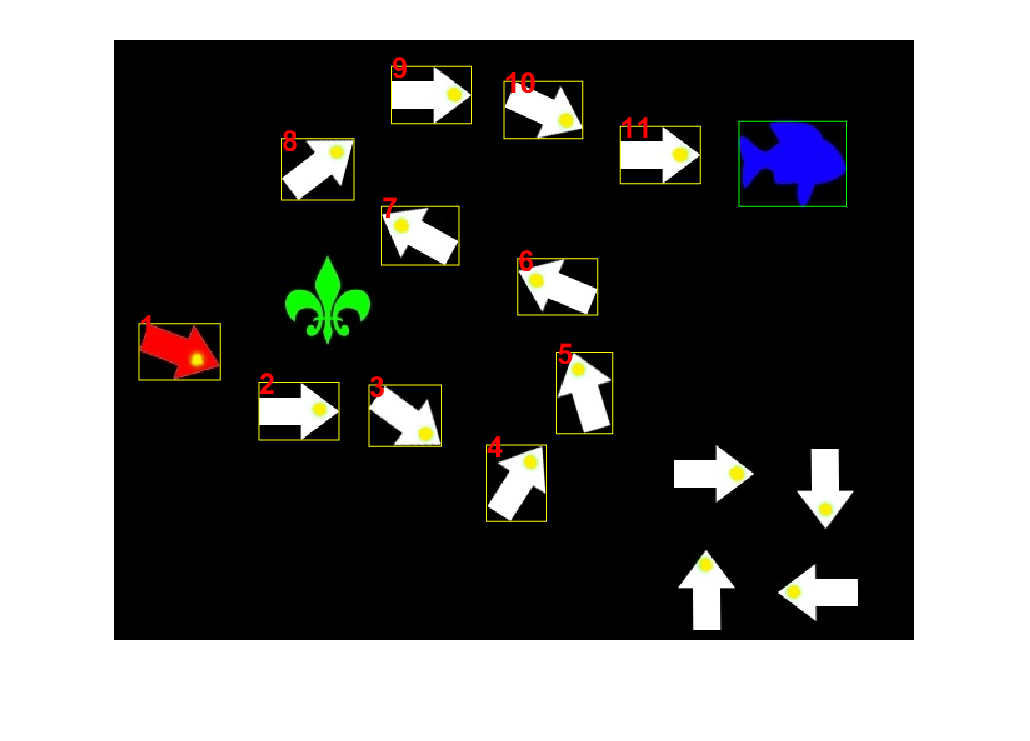
\includegraphics[width=0.75\linewidth]{Lab 4/MediumVisualSolution.png}
    \caption{Visualisation of medium treasure hunting}
    \label{fig:MediumVisualSolution}
\end{figure}

\begin{figure}[ht]
    \centering
    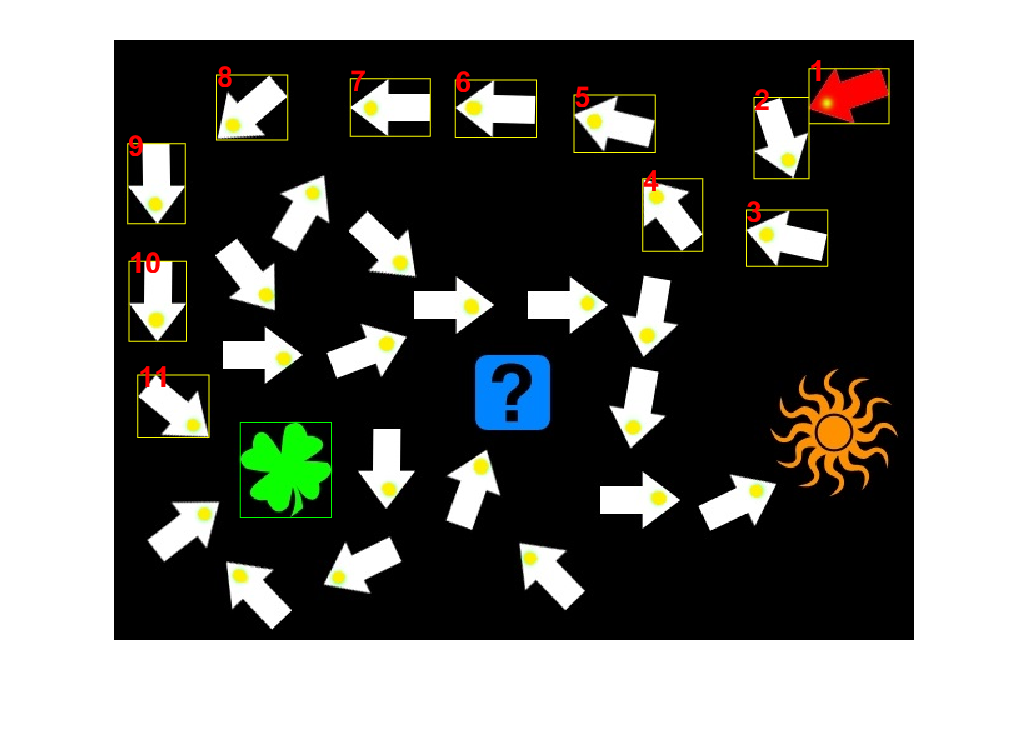
\includegraphics[width=0.75\linewidth]{Lab 4/HardVisualSolution.png}
    \caption{Visualisation of hard treasure hunting}
    \label{fig:HardVisualSolution}
\end{figure}

As can be seen in \ref{fig:HardVisualSolution}, the path is numbered in order and then the treasure is highlighted with a rectangle and no number. In this case, the treasure is a four leaf clover.

\clearpage
\section{Task 5: Image Classification with a Convolutional Neural Network (CNN)}\label{CNNImageClassifier}
\subsection{Designing and Training a CNN}
The predominant CNN architecture in this task is based off \textit{LeNet-5}, which has played a significant role in the development of deep learning, particularly in the field of computer vision. We were given a sample \textit{LeNet-5} architecture in the lab sheet of which the training progress can be seen in figure \ref{fig:BaseCNNTrainingProgress}. The performance metrics from this baseline model can be seen in table \ref{tab:BaselinePerformanceMetrics}.

\begin{table}[ht]
    \begin{center}
      \caption{Table of performance metrics from baseline model}
      \label{tab:BaselinePerformanceMetrics}
      \begin{tabular}{l|r} % <-- Alignments: 1st column left, 2nd middle and 3rd right, with vertical lines in between
        \textbf{Metric} & \textbf{Score}\\
        % $\alpha$ & $\beta$ & $\gamma$ \\
        \hline
        Accuracy & 0.6270\\
        Precision & 0.6294\\
        Recall & 0.6270\\
        F1 score & 0.6282\\
      \end{tabular}
    \end{center}
  \end{table}

\begin{figure}[ht]
    \centering
    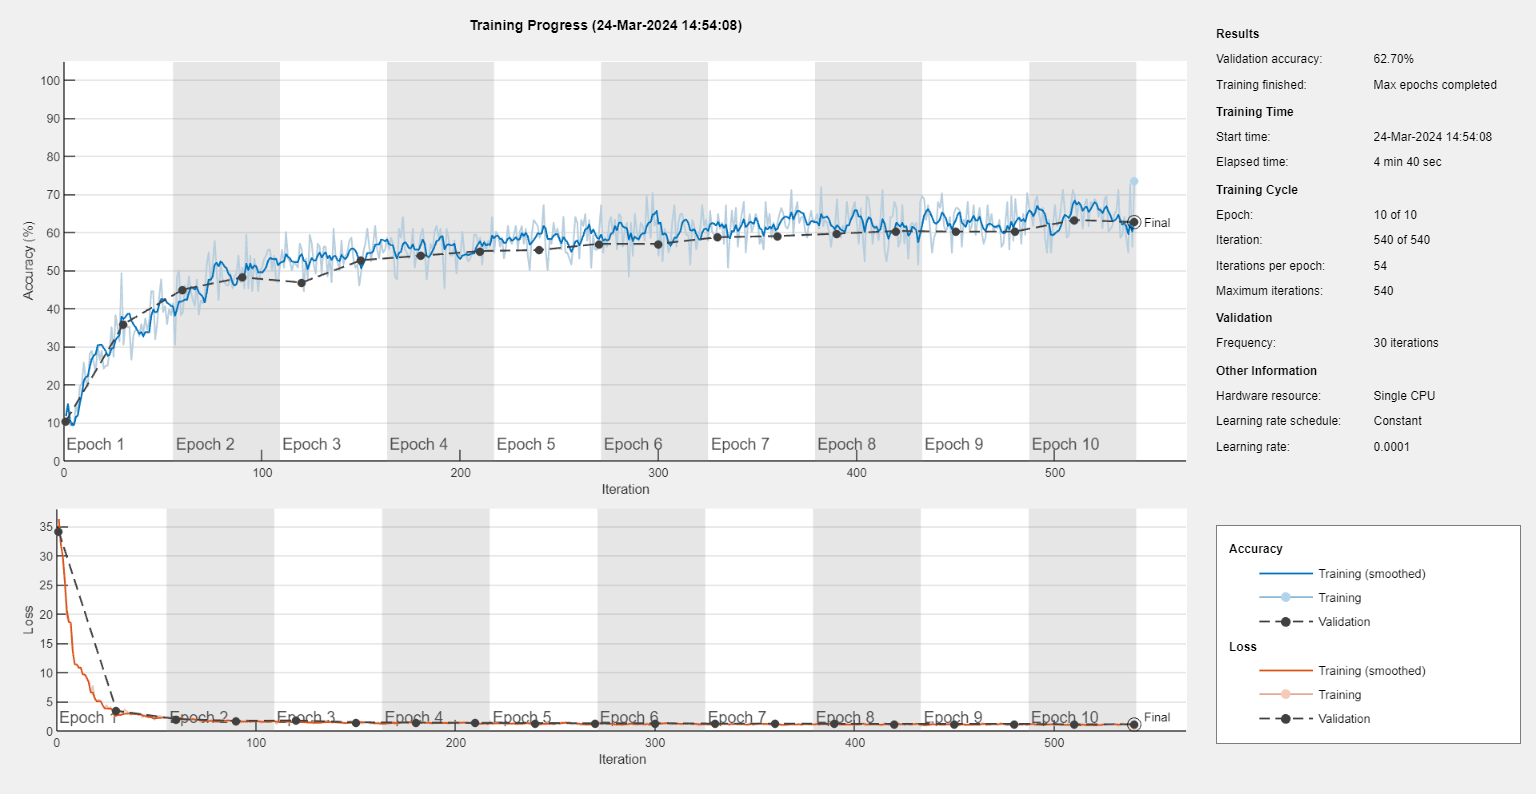
\includegraphics[width=0.75\linewidth]{Lab 5/BaseCNNTrainingProgress.png}
    \caption{Training progress seen from unaltered CNN architecture}
    \label{fig:BaseCNNTrainingProgress}
\end{figure}

As can be seen in figure \ref{fig:BaseCNNTrainingProgress} and table \ref{tab:BaselinePerformanceMetrics}, the performance metrics of the baseline model point to this model not being very good. 

\subsection{Improving the performance of the CNN Algorithm}
The next part of this task involved improving the performance of the CNN  through a number of different methods.
\subsubsection*{Regularisation techniques}
The suggested approach in the lab sheet for this part of the task was to combine \textit{L1} and \textit{L2} regularisation. This is called \textit{elastic net regularisation} and is supposed to improve the generalisation capability of the model. However, it is not used very often as it introduces an extra hyperparameter which demands meticulous tuning. With this is mind, the first method I chose to try to improve the performance of the classifier was \textit{L2 regularisation}. The main reason I chose this over \textit{L1 regularisation} is because \textit{L2 regularisation} is more stable than \textit{L1 regularisation}.

Having chosen \textit{L2 regularisation}, I had to decide on what value the ``WeightL2Factor" hyperparameter would take for each fully connected layer of the CNN. I decided to use Latin Hypercube Sampling \cite{LHS} to help me choose the best combination. This led to results which were not as good as hoped for, with a very slight decrease in accuracy as can be seen in table \ref{tab:L2RegularisationPerformanceMetrics}. The best lambda values were: 0.313383, 0.423196, 0.634686. These values were used in the ``fullyConnectedLayer()" functions seen in the base version of the CNN architecture respectively. The optimisation can be seen in listing \ref{LHS_optimisation}.

\begin{table}[ht]
  \begin{center}
    \caption{Table of performance metrics from L2 Regularisation model}
    \label{tab:L2RegularisationPerformanceMetrics}
    \begin{tabular}{l|r} % <-- Alignments: 1st column left, 2nd middle and 3rd right, with vertical lines in between
      \textbf{Metric} & \textbf{Score}\\
      \hline
      Accuracy & 0.6157\\
      Precision & 0.6173\\
      Recall & 0.6157\\
      F1 score & 0.6165\\
    \end{tabular}
  \end{center}
\end{table}

The next regularisation technique I tried to implement was \textit{dropout}. This method initially gave me awful accuracy but I then decreased the dropout rate of the dropout layers from 0.5 to 0.1 and performance then only dropped a little from how it was pre-regularisation techniques. These performance metrics can be seen in \ref{tab:DropoutRegularisationPerformanceMetrics}.

\begin{table}[ht]
    \begin{center}
      \caption{Table of performance metrics from dropout regularisation model}
      \label{tab:DropoutRegularisationPerformanceMetrics}
      \begin{tabular}{l|r} % <-- Alignments: 1st column left, 2nd middle and 3rd right, with vertical lines in between
        \textbf{Metric} & \textbf{Score}\\
        % $\alpha$ & $\beta$ & $\gamma$ \\
        \hline
        Accuracy & 0.5857\\
        Precision & 0.5862\\
        Recall & 0.5857\\
        F1 score & 0.5859\\
      \end{tabular}
    \end{center}
  \end{table}

Given both of these regularisation techniques implemented in different ways led to the model being less accurate than before they were implemented, I decided to leave them out of future models. They did not seem to be effective for this problem.

\subsubsection*{Activation functions}
Using this method to optimise the CNN architecture was much easier to implement and it also led to better results immediately. For the first activation function all I did was add a \textit{Rectified Linear Units} (ReLU) activation function after each convolution layer. The training progress graph for this can be seen in figure \ref{fig:ReLUActivationTrainingProgress}. The performance metrics from this can be seen in table \ref{tab:ReLUActivationPerformanceMetrics}

\begin{table}[ht]
    \begin{center}
      \caption{Table of performance metrics from ReLU activation function model}
      \label{tab:ReLUActivationPerformanceMetrics}
      \begin{tabular}{l|r} % <-- Alignments: 1st column left, 2nd middle and 3rd right, with vertical lines in between
        \textbf{Metric} & \textbf{Score}\\
        % $\alpha$ & $\beta$ & $\gamma$ \\
        \hline
        Accuracy & 0.7123\\
        Precision & 0.7214\\
        Recall & 0.7123\\
        F1 score & 0.7124\\
      \end{tabular}
    \end{center}
  \end{table}

\begin{figure}[ht]
    \centering
    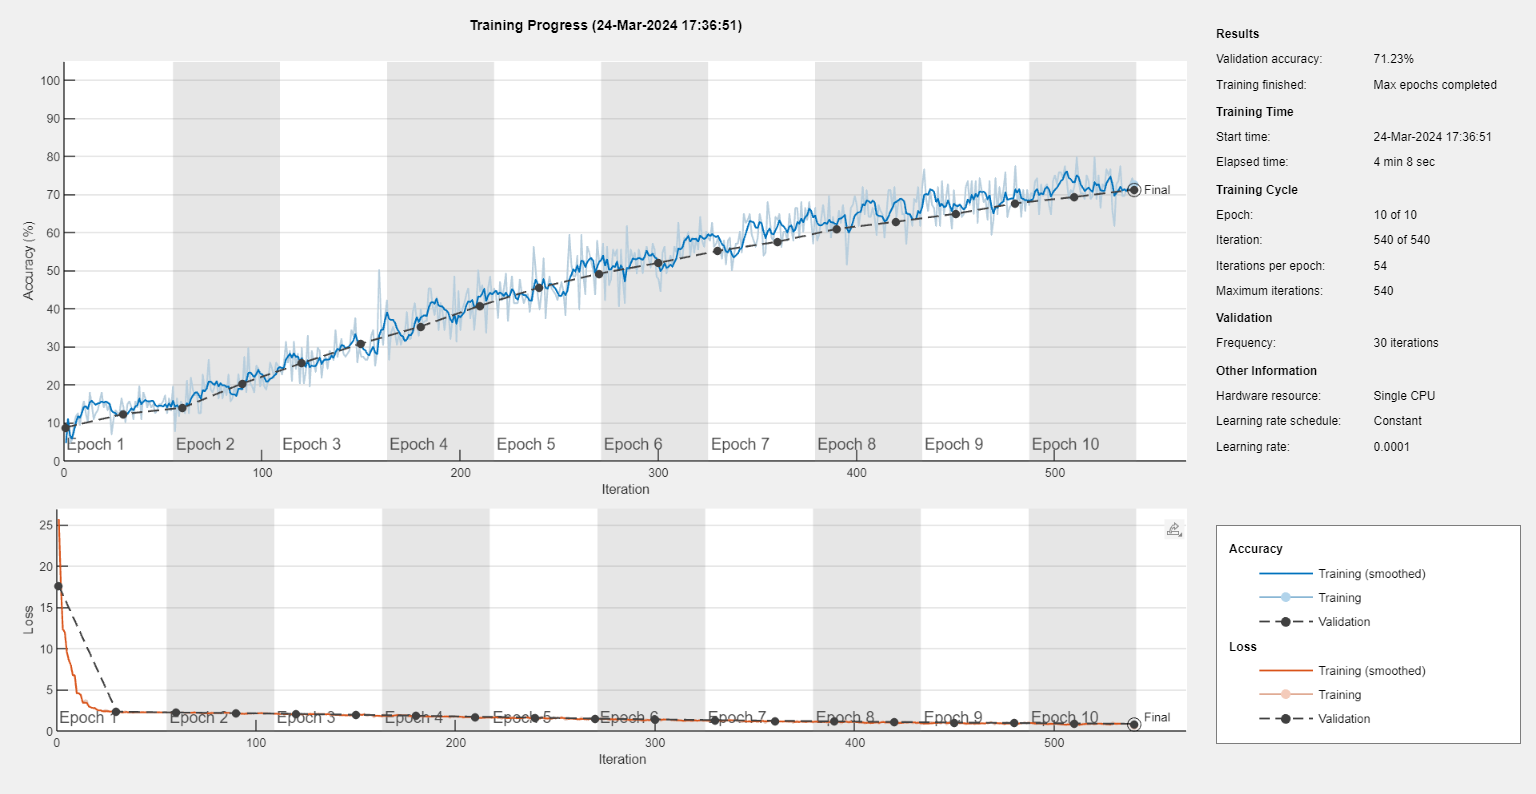
\includegraphics[width=1\linewidth]{Lab 5/ReLUActivationTrainingProgress.png}
    \caption{Training Progress graph from implementing activation function after each convolution layer}
    \label{fig:ReLUActivationTrainingProgress}
\end{figure}

One trend we see in figure \ref{fig:ReLUActivationTrainingProgress} is that the accuracy doesn't flatten out after 3 or 4 epochs as it did with previous training progress graphs. This could be attributed to several things, but overall is down to the \textit{ReLU} activation function enhancing the power of neural networks through non-linearity and promoting more stable and efficient training dynamics \cite{ReLU-Brownlee}. This facilitates better representation learning. 

For the second activation function I decided to use the \textit{Sigmoid} activation function which led to a dramatic fall in accuracy, as seen in table \ref{tab:SigmoidActivationPerformanceMetrics}. Based off the performance of the two activation functions seen here, I opted to add the \textit{ReLU} activation function to my final CNN architecture seen in listing \ref{Optimal_LeNet5} due to the significant increase in model accuracy it achieved.

\begin{table}[ht]
    \begin{center}
      \caption{Table of performance metrics from Sigmoid activation function model}
      \label{tab:SigmoidActivationPerformanceMetrics}
      \begin{tabular}{l|r} % <-- Alignments: 1st column left, 2nd middle and 3rd right, with vertical lines in between
        \textbf{Metric} & \textbf{Score}\\
        \hline
        Accuracy & 0.16\\
        Precision & 0.1337\\
        Recall & 0.16\\
        F1 score & 0.1457\\
      \end{tabular}
    \end{center}
  \end{table}

\subsubsection*{CNN architecture exploration}
In this section my attention was drawn to the \textit{AlexNet} architecture mentioned in the lab sheet. Upon further reading \cite{AlexNet, DeepLearningCNN}, I learnt that it is regarded as a big part of why CNN has become such a popular deep learning architecture.

When making my \textit{AlexNet} model there were a number of hyperparameters I decided to adjust from the model architecture seen in \cite{AlexNet}. The original \textit{AlexNet} architecture was designed for handling an input much larger than the one in this lab. Therefore, I decided to reduce some of the hyperparameters which came after this too, including the size of the filters in the first convolutional layer. The code I wrote to build the model is seen in listing \ref{AlexNet_with_hyperparameters}.

Aside from there being more layers in the \textit{AlexNet} than the \textit{LeNet-5} design, the pooling method used was also different. In \textit{LeNet-5}, \textit{average pooling} is used whereas \textit{max pooling} \cite{MATLABmaxPoolingLayer} is used in \textit{AlexNet}. \textit{Max pooling} is the most popular type of pooling and it just takes the max value in the pooling window. This window is slid over the input and the max value in the window at each position is taken. We only need to specify the window size and stride. With the pooling function used as it is in code seen in listing \ref{AlexNet_with_hyperparameters}, each time it is used, the size of the feature map is halved. Downsampling the feature map whilst keeping the important information is the main use of pooling. For this task, \textit{max pooling} is better due to the data being composed of black and white images, and \textit{max pooling} being better at preserving important features.

Whilst training the model, I noticed the \textit{AlexNet} model I had built took a lot longer than the original \textit{LeNet-5} model. This is due to model complexity and the fact that \textit{AlexNet} was actually built to take advantage of parallel computing resources, which I did not have access to when training the network.

The results that the \textit{AlexNet} model produced were far superior to what we'd seen up to this point, so it could be argued that it was worth the long wait for the model to train.

\begin{table}[ht]
  \begin{center}
    \caption{Table of performance metrics from AlexNet model}
    \label{tab:AlexNetPerformanceMetrics}
    \begin{tabular}{l|r} % <-- Alignments: 1st column left, 2nd middle and 3rd right, with vertical lines in between
      \textbf{Metric} & \textbf{Score}\\
      % $\alpha$ & $\beta$ & $\gamma$ \\
      \hline
      Accuracy & 0.9907\\
      Precision & 0.9907\\
      Recall & 0.9907\\
      F1 score & 0.9907\\
    \end{tabular}
  \end{center}
\end{table}

\begin{figure}[ht]
  \centering
  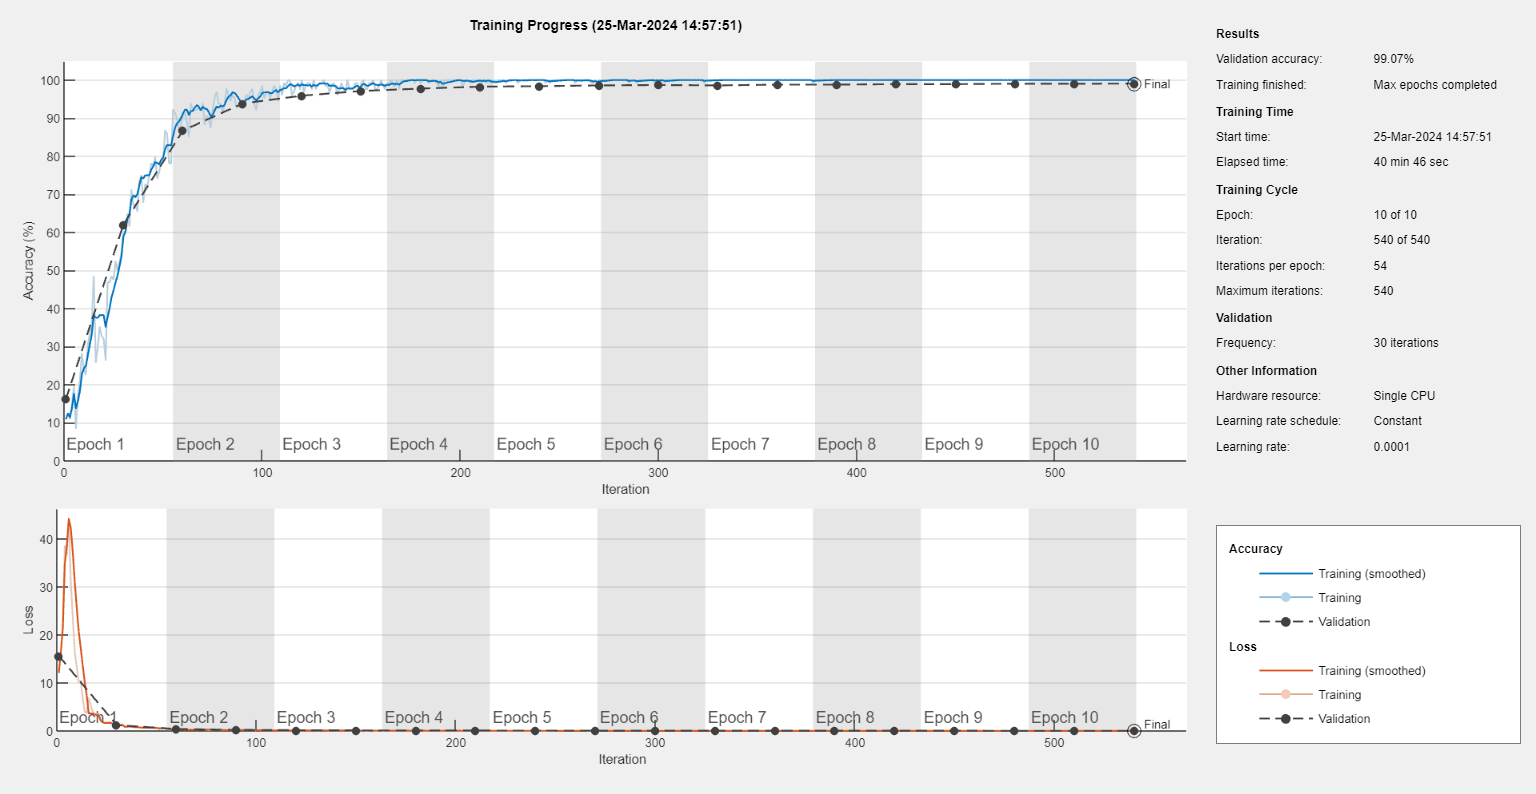
\includegraphics[width=1\linewidth]{Lab 5/OriginalAlexNetTrainingProgress.png}
  \caption{Training Progress of original AlexNet model}
  \label{fig:OriginalAlexNetTrainingProgress}
\end{figure}

\subsubsection*{Hyperparameter tuning}
For this section, I systematically varied the hyperparameters on the orginal model we were given. The first model I built was less accurate than the second, the structure of it can be seen in the code in figure \ref{subOptimal_LeNet5}. My main takeaway from this part of the task was no matter how much training of a model is done, it doesn't matter if the architecture is unsuitable. This can be seen in figure \ref{fig:HyperparameterOKresultTrainingProgress}. The model accuracy is seen to level out after four or five epochs. We end with performance metrics seen in table \ref{tab:SubOptimalHyperparametersMetrics}.

\begin{table}[ht]
  \begin{center}
    \caption{Table of performance metrics from neural network with sub-optimal hyperparameters}
    \label{tab:SubOptimalHyperparametersMetrics}
    \begin{tabular}{l|r} % <-- Alignments: 1st column left, 2nd middle and 3rd right, with vertical lines in between
      \textbf{Metric} & \textbf{Score}\\
      % $\alpha$ & $\beta$ & $\gamma$ \\
      \hline
      Accuracy & 0.6680\\
      Precision & 0.6729\\
      Recall & 0.6680\\
      F1 score & 0.6704\\
    \end{tabular}
  \end{center}
\end{table}

\begin{figure}[ht]
  \centering
  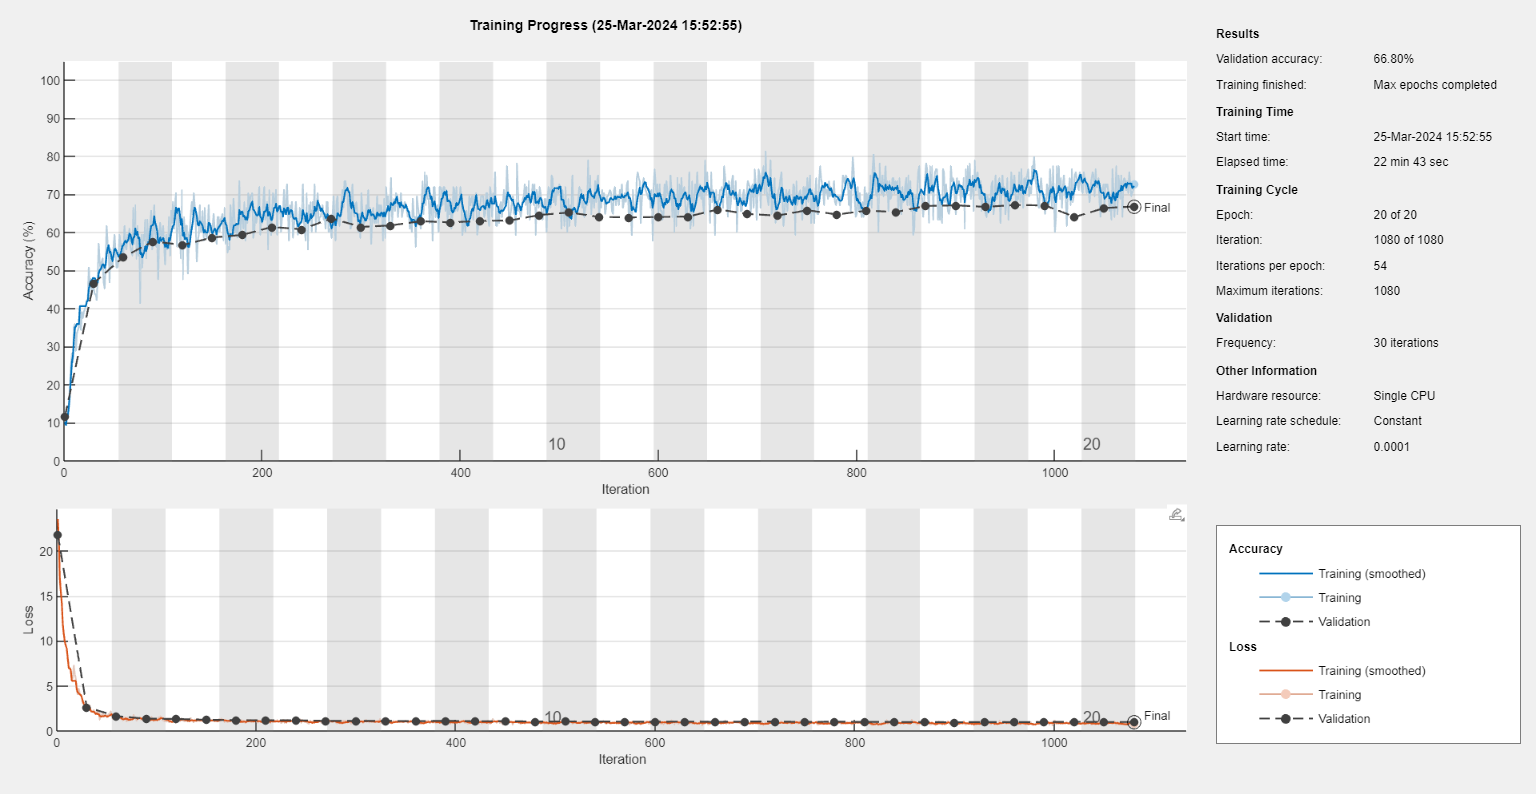
\includegraphics[width=1\linewidth]{Lab 5/HyperparameterOKresultTrainingProgress.png}
  \caption{Training process of neural network with sub-optimal hyperparameters}
  \label{fig:HyperparameterOKresultTrainingProgress}
\end{figure}

Due to the accuracy metric levelling off after 5 epochs as seen in figure \ref{fig:HyperparameterOKresultTrainingProgress}, we can put the increase in accuracy relative to our original model down to the other hyperparameters being changed. Upon experimenting with many different combinations of hyperparameters, I found there to be a low ceiling without using a \textit{ReLu} activation function. This ceiling is illustrated by table \ref{tab:SubOptimalHyperparametersMetrics} and figure \ref{fig:HyperparameterOKresultTrainingProgress}. 

The optimised model I have presented in listing \ref{Optimal_LeNet5} has a very high accuracy and takes a relatively short time to train. I designed it off the back of the original model given to us in the lab and added a few features, as well as optimising some of the hyperparameters using Latin hypercube sampling \cite{LHS}. This gave me the results seen in figure \ref{fig:OwnCNNTrainingProcess} and in table \ref{tab:OwnCNNPerformanceMetrics}.

Regarding the filter count of the different layers seen in the network, the theory \cite{DeepLearningCNN} states that ``using more filters results in a more powerful model but at the risk of overfitting due to increased parameter count''. Again, there is no single correct place to start as previously mentioned, but after testing a dozen different combinations, I settled with what is seen in listing \ref{Optimal_LeNet5}. When I ran the model with these parameters, the accuracy was very high.

\begin{table}[ht]
  \begin{center}
    \caption{Table of performance metrics from edited LeNet-5 model}
    \label{tab:OwnCNNPerformanceMetrics}
    \begin{tabular}{l|r} % <-- Alignments: 1st column left, 2nd middle and 3rd right, with vertical lines in between
      \textbf{Metric} & \textbf{Score}\\
      % $\alpha$ & $\beta$ & $\gamma$ \\
      \hline
      Accuracy & 0.9807\\
      Precision & 0.9809\\
      Recall & 0.9807\\
      F1 score & 0.9808\\
    \end{tabular}
  \end{center}
\end{table}

\begin{figure}[ht]
    \centering
    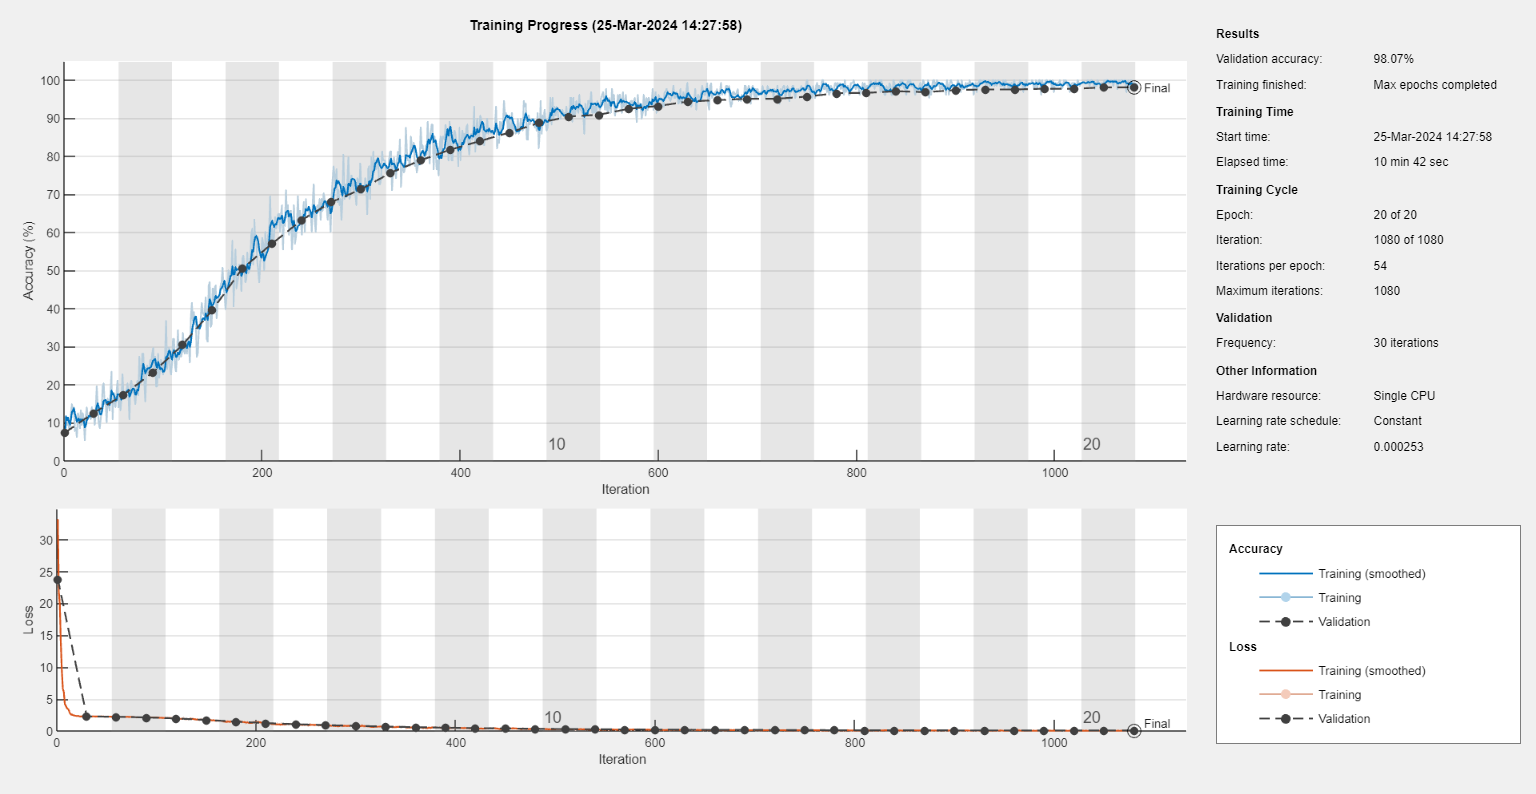
\includegraphics[width=1\linewidth]{Lab 5/OwnCNNTrainingProcess.png}
    \caption{Training progress seen for optimised parameters model using Latin Hypercube Sampling}
    \label{fig:OwnCNNTrainingProcess}
\end{figure}

The results seen in table \ref{tab:OwnCNNPerformanceMetrics} and figure \ref{fig:OwnCNNTrainingProcess} were very good compared to the orginal model and came as a result of some simple changes. Two of these, the learning rate and number of epochs, come in the training options. Increasing the number of epochs from ten to 20 led to an increase in accuracy of about 8\%. This led me to the conclusion that the training hyperparameters will only make a difference if the model is structured well to begin with. One very important addition to the architecture was the activation function. This increased accuracy drastically from when it was not there.

The accuracy is still slightly less than that seen using the enhanced \textit{AlexNet} network seen in listing \ref{AlexNet_with_hyperparameters}. However, this could easily be the other way round if a different random seed was used. Also, the \textit{AlexNet} model took a lot longer to train, despite being trained over half as many epochs and at a lower learning rate.

\clearpage
\subsection{Ethics in Computer Vision}
Ethics is a very important part of computer vision which needs to be considered every time computer vision is used in real-life scenarios, whether that be in image classification, detection, segmentation, or other areas. Ethics issues become very apparent when we consider equality, diversity and inclusion (EDI) in particular. Discussed here are the challenges machine vision pose, why we benefit from identifying these challenges, and potential solutions. 

\subsubsection*{Bad data}
After consulting the relevant literature it became apparent that many popular facial recognition models have varying performance capabilities across sex and ethnic groups. Some of these performance gaps are so large they lead to false positives being up to twice as likely for some demographics compared to others \cite{SernaImprovingFaceRepresentation}. Another more specific example of this is seen with a Nikon camera, where a Taiwanese-American family found that their camera could not correctly identify whether they were blinking or not \cite{NikonBlinkDetection}. 

There is limited literature on the matter but most of the literature seen put the discrimination down to ``bad data'', or more specifically ``non-representative training data'' \cite{BadDataMedium}. The general consensus is that image classification models regarding people are predominantly trained on caucasians and therefore struggle to classify other ethnicities accurately. Perhaps the most alarming example of discrimination due to training data is the case seen in a study to investigate object detection inequity among different skin tones, with a higher success rate found detecting lighter skin tones \cite{WilsonInequityObjectDetection}. This bias and discrimination problem is not limited to machine vision but can also be seen in other areas of machine learning \cite{BiasInMLHawaii}.

So, perhaps one way to help solve the issue of bias in machine vision is to have models which are put to use in real-life scenarios be trained on ``good'', representative data. This can come partly through data-processing and cleaning up training data. Another potential solution to this problem is to use discrimination-aware training methods like \textit{sensitive-loss}. An example of this being put to use sees the model with \textit{sensitive-loss} added outperform the models without both in terms of accuracy and in fairness metrics \cite{SernaImprovingFaceRepresentation}.

\subsubsection*{Lack of algorithmic transparency}
Another reason why certain parts of machine vision could pose an ethical problem is due to the lack of algorithmic transparency and explainability. Neural networks like those seen in the task under section \ref{CNNImageClassifier} are often referred to as ``black box'' because it is difficult to understand how they make their decisions. There are a number of reasons why this is a concern. One reason is that it can be difficult to trust these models if we don't understand how they work, especially in important applications where the stakes are high. An example of this in machine vision could be in driverless cars. This problem is one of the main factors contributing to why driverless cars aren't being rolled out on a commercial level just yet.

To bring this argument to life, how does a driverless car decide, if these are the only two possible outcomes, whether to run over an elderly person or a school child? Is the child's life more valuable than the elderly person's? It is an ethical concern that this kind of decision would have to be made partly by a computer vision sub-system on a car where nobody fully understands the machine learning algorithm on board. The lack of algorithmic transparency is a well-known issue in machine learning in general and there are many ideas for a solution. 

One possible solution is to use methods that can provide explanations on how they work and how they produce certain results. This can be split into two categories, \textit{intrinsic} and \textit{post-hoc}. \textit{Intrinsic} are those with transparent model design, this could be done through using simple or interpretable algorithms and avoiding black-box techniques. \textit{Post-hoc} refers to using explanations after the model is trained such as visualisation or feature importance methods. 

Another popular solution for this problem among industry leading experts is known as model lifecycle documentation. This is what it sounds like, and involves documenting the model lifecycle from data collention to deployment and monitoring. Documentation can help when assessing the quality of the data used and the model itself. It can also help stakeholders not from a technical background to understand what the model is doing along with any associated risks and benefits on society.

\subsubsection*{Inadequate regulation and oversight}
This final issue is an all-encompassing one. Machine vision models need to be regulated in order for the general population to be safe. Just like there is the Driver and Vehicle Standards Agency in the UK to protect people on the road, there must be an agency to protect people from machine vision algorithms which they may be interacting with. 

There has been much international dicussion including the AI safety summit at Bletchley Park in 2023 \cite{AIsafetySummit} surrounding regulation of AI risks, which machine vision comes under. The regulation could be used to enforce improvements to bias models to ensure they are not biased.

\subsubsection*{Conclusion}
There is still a lot of work to be done to ensure that all ethical concerns surrounding machine vision and equality can be met. If the right people in the right positions take ownership of the issues then all this technology can be put to good use. This should be straightforward but there is a large risk if the authorities don't act correctly on the matter.

\clearpage
\section{Bibliography}
\printbibliography

\clearpage
\appendix
\section{Exercise 2 code}
\lstset{style=mystyle}
\lstinputlisting[caption={Script for exercise 2}, label=Ex2MATLABscript, style=mystyle]{Lab 2/Lab_2.m}

\clearpage
\section{Exercise 3 code}
\lstset{style=mystyle}
\lstinputlisting[caption={Script for exercise 3}, label=Ex3MATLABscript, style=mystyle]{Lab 3/Lab3.m}

\clearpage
\section{Exercise 4 code - Arrow finding}
\lstset{style=mystyle}
\lstinputlisting[caption={Main script for exercise 4}, label=Ex4MATLABscript, style=mystyle]{Lab 4/treasure_hunting_all.m}

\lstset{style=mystyle}
\lstinputlisting[caption={Arrow finder function}, label=arrowFinderFunction, style=mystyle]{Lab 4/arrow_finder.m}

\lstset{style=mystyle}
\lstinputlisting[caption={Yellow spot finder function}, label=yellowFinderFunction, style=mystyle]{Lab 4/yellowFinder.m}

\lstset{style=mystyle}
\lstinputlisting[caption={Next object finder function}, label=nextObjectFinderFunction, style=mystyle]{Lab 4/next_object_finder.m}


\clearpage
\section{Exercise 5 code - CNNs}

\lstset{style=mystyle}
\lstinputlisting[caption={LHS optimisation on L2 regularisation}, label=LHS_optimisation, style=mystyle]{Lab 5/LHS_optimisation.m}

\lstset{style=mystyle}
\lstinputlisting[caption={AlexNet code with hyperparameters}, label=AlexNet_with_hyperparameters, style=mystyle]{Lab 5/AlexNet_with_hyperparameters.m}

\lstset{style=mystyle}
\lstinputlisting[caption={Code for sub-optimal LeNet-5 CNN}, label=subOptimal_LeNet5, style=mystyle]{Lab 5/subOptimal_LeNet5.m}

\lstset{style=mystyle}
\lstinputlisting[caption={Code for optimal LeNet-5 CNN}, label=Optimal_LeNet5, style=mystyle]{Lab 5/Optimal_LeNet5.m}

\end{document}
